% Body of paper at ch2/papers/exp_vocab/main.tex
% Standalone preamble stripped; \input from the chapter wrapper.
\graphicspath{{ch2/papers/exp_vocab/}}
% Custom commands preserved from the original preamble:
\providecommand{\meCDI}{\textsc{corpus-CDI}}



\section{Introduction}

Large language models (LLMs) have shown that a general-purpose architecture trained on large text corpora can acquire rich syntactic and semantic knowledge \citep{brown2020language, devlin2019bert, touvron2023llama}. Beyond their impact on NLP applications \citep{bommasani2021opportunities}, LLMs provide scalable tools for testing theories of early language acquisition \citep{dupoux2018cognitive, evanson2023language, lavechin2022reverse, apidianaki2024language, hu2025language}. In particular, they offer a controlled way to investigate the long-standing hypothesis that children bootstrap into language learning by accumulating statistics from linguistic input \citep{saffran1996statistical}.

A central challenge when applying LLMs as models of the early language learner is establishing valid \emph{quantitative} comparisons between the learning trajectories of real children and those of LLMs fed with comparable data. For instance, it has been claimed that LLMs require significantly more input data than children to reach the same level of performance \citep{frank2023bridging}. But measuring this 'data gap' depends critically on developing sound metrics that can be applied consistently to both human learners and computational models.  


We focus on measures of vocabulary, as there is a wealth of developmental data that provides human side of the comparison. Previous work has primarily explored two approaches for evaluating vocabulary in models: (i) \textbf{familiarity metrics}, which exploit LLMs' probabilistic outputs (e.g., surprisal or word–pseudoword preference) to probe lexical knowledge \citep{chang2022word, ma2025babysit, lavechin2025simulating}; and (ii) \textbf{cross-modal matching}, which assesses word–referent grounding using multimodal training and behavioral benchmarks \citep{vong2024grounded, tan2024devbench, nikolaus2021modeling}, analogous to looking-while-listening paradigms in children \citep{swingley2011looking}. While informative, familiarity metrics often rely on limited behavioral data, and cross-modal methods require multimodal input unavailable to unimodal language models. Also, neither of them has focused on expressive vocabulary. 



To overcome these limitations and enable large-scale, quantitative comparison with child vocabulary, we introduce \meCDI{}, a benchmark that aligns model generations with children's expressive vocabulary. \meCDI{} calibrates three key dimensions: (1) training exposure, scaled from 6 to 36 months based on daylong recordings \citep{cristia2019child}; (2) cumulative generated word count, matched to children’s monthly word production rates; and (3) evaluation vocabulary, matched in part-of-speech categories and frequency distribution to the CDI word list \citep{frank2017wordbank}.



Using \meCDI{}, we evaluate character-level LSTMs and Transformers trained on child-directed speech (CDS) and audiobook transcripts.
We assess vocabulary acquisition across three complementary dimensions: lexical diversity (type-token ratio), word form accuracy (non-word rate), and vocabulary size (\meCDI{} score). Our analyses reveal that language models diverge from children in critical ways: models show excessive lexical diversity, minimal improvement in word form accuracy, and slower vocabulary growth. Frequency analyses further indicate that these gaps stem from long-tail truncation: low-frequency words are severely underrepresented in model acquisition, while high-frequency function words are overrepresented relative to children’s productions.

% These results suggest that optimizing for optimizing for next-word prediction alone is insufficient to reproduce the structure and dynamics of early lexical development. Instead, successful modeling of human vocabulary growth likely requires inductive biases and learning signals that more closely reflect the multimodal, social, and cognitively constrained nature of child learning.

% Overall, \meCDI{} provides a new evaluation framework for measuring expressive vocabulary growth in language models in a way that is directly comparable to child development. By aligning exposure, production, and evaluation along developmentally grounded dimensions, this benchmark enables a more precise assessment of where and why current models succeed or fail as cognitive models of language acquisition.



\begin{comment}
---- extended intro

Research into Large language models (LLMs) have demonstrated that a generic learning architecture fed with a static corpus of text can learn rich syntactic and semantic properties of a language (ref). Apart from disrupting natural language processing and associated technologies (ref), these models had also considerable impact on cognitive science: %For one, it revived long-standing controversies regarding the nature/nurture debate on the origin of language (ref). 
it provided powerful computational tools for implementing and testing theories of human language acquisition in children \citep{dupoux2018cognitive,evanson2023language,hu2024findings,charpentier2025babylm,apidianaki2024language}. LLMs can indeed be seen as the computational implementation of the 'statistical learning' theory according to which children bootstrap into language learning through building a probabilistic model of the language input that they receive from their language environment \citep{saffran1996statistical}. 


However, a considerable stumbling block for the direct application of LLMs as models of the early language learner is the possibility of making valid quantitative comparisons between the learning curves of real children and those of LLMs fed with comparable data. For instance, it has been claimed that LLMs require significanly more input data than children to reach the same level of performance \citep{frank2023bridging}. But the measure of such 'data gap' is critically dependant on the developmment of sound metrics that enable to measurment of language outcomes in both humans and machines. 

In this paper, we focus on measures of vocabulary, as there is a wealth of developmental data which provides the human side of the comparison. We distinguish three methods to evaluate vocabulary that can be applied to machines and children alike: \textit{familiarity metrics}, \textit{cross-modal matching}, and \textit{production metrics}.

Familiarity metrics use the fact that LLMs are probabilistic models; at each time step, they output a probability distribution of next tokens based on the previous context. Several papers have therefore used surprisal \citep{chang2022word,ma2024babysit} to evaluate whether models can correctly predict the probability of a word given context, or whether, in the absence of context 'prefer' real words like 'brick' to orthographically legal pseudo-words like 'blick' \citep{lavechin2023babyslm}. Similar word-nonword preference techniques exist in real children (Ngon et al; other refs), but the data is very scarse, making it difficult to compare the vocabulary growth quantitatively. 


Cross-modal matching evaluate word-object mappings through multimodal tasks \citep{nikolaus2021modeling,vong2024grounded,tan2024devbench}, the equivalent of looking while listening in children (). This method gives vary comparable scores between machines and children, but unfortunately it cannot be applied to unimodal (language only) models. 


Finally, production metrics use the capability of next token prediction LLMs to be turned to 'speak', ie, to generate language on their own. The generated corpus can therefore be analysed with the same tools that are use to analyse children's production, enabling a quantitative comparison between children and models. In order to make a valid comparison, however, it is important to match the input that is used to train the model to the input available to children. This is the method we use in this paper. 



We introduce \meCDI{}, a benchmark that enables direct comparison between child expressive vocabulary and language model generation. \meCDI{} calibrates three key dimensions: (1) training exposure, scaled to developmental stages from 6 to 36 months based on daylong recordings \citep{cristia2019child}; (2) cumulated generated word count, calibrated to children’s monthly word production rates; and (3) calibrated test vocabulary, matched in part of speech and frequency distribution to the CDI word list (ref).

With \meCDI{}, we evaluate character-level LSTMs and Transformers trained on two types of input: naturalistic child-directed speech and audiobook transcripts. We assess vocabulary acquisition across three complementary dimensions: lexical diversity (type-token ratio), word form accuracy (non-word rate), and vocabulary size (\meCDI{} score). Our analyses reveal divergences from children: models show excessive lexical diversity, minimal improvement in word form accuracy, and sub-linear vocabulary growth that lacks the characteristic acceleration of human development. Frequency analyses suggest that these gaps are driven by long-tail truncation, whereby low-frequency words are underrepresented in model output, while high frequency function words are overrepresented compared to children.
\end{comment}



\begin{comment}
---- old intro

Large language models (LLMs) have demonstrated remarkable linguistic capabilities, from syntactic judgment \citep{warstadt2019neural} to semantic inference \citep{yang2024exploring}. These successes make LLMs as computational tools for testing theories of human language acquisition \citep{dupoux2018cognitive}. However, this requires carefully designed benchmarks that enable direct comparisons between model behavior and child language development.



Existing approaches to evaluating vocabulary acquisition in models fall into two categories. \textit{Implicit methods} infer word knowledge indirectly through surprisal \citep{chang2022word,ma2024babysit} or zero-shot lexical decision tasks \citep{lavechin2023babyslm}. While correlated with child vocabulary measures, these methods do not capture productive vocabulary, i.e., the words children actually produce. \textit{Explicit methods} evaluate word-object mappings through multimodal tasks \citep{nikolaus2021modeling,vong2024grounded,tan2024devbench}, but rely on pre-trained subword tokenizers that introduce evaluation gaps: models never generate complete word forms as discrete units, preventing direct comparison with child production.

Modeling developmental trajectories presents additional challenges. Some studies use training checkpoints to simulate developmental time \citep{chang2022word,evanson2023language}, while others vary total data exposure \citep{lavechin2023babyslm}. Both approaches fail to fully capture children's learning conditions: checkpoint-based training repeatedly exposes models to identical data, whereas children experience progressively varied input \citep{rasanen2024age}; data-size approaches control input quantity but leave output production and evaluation frequencies uncalibrated.

We introduce \meCDI{}, a benchmark that enables direct comparison between child expressive vocabulary and language model generation. \meCDI{} calibrates three key dimensions: (1) training exposure, scaled to developmental stages from 6 to 36 months based on daylong recordings \citep{cristia2019child}; (2) generation quantity, matched to children’s monthly word production rates; and (3) evaluation frequency, where CDI words' distributions mirror their occurrence in child-directed speech.

With \meCDI{}, we evaluate character-level LSTMs and Transformers trained on two types of input: naturalistic child-directed speech and audiobook transcripts. We assess vocabulary acquisition across three complementary dimensions: lexical diversity (type-token ratio), word form accuracy (non-word rate), and vocabulary size (\meCDI{} score). Our analyses reveal divergences from children: models show excessive lexical diversity, minimal improvement in word form accuracy, and sub-linear vocabulary growth that lacks the characteristic acceleration of human development. Frequency analyses suggest that these gaps are driven by long-tail truncation, whereby low-frequency words are underrepresented in model output.
\end{comment}



\section{Related Work}

% \subsection{Developmental Trajectories Across Linguistic Levels}
\subsection{Developmental Trajectories}

Prior work has examined the alignment between language model learning and child language development across multiple linguistic levels. A key challenge is mapping model training onto corresponding developmental milestones. Early studies used training checkpoints as proxies for age, tracking when models acquire words \citep{chang2022word} or syntactic structures \citep{evanson2023language}. However, these approaches repeatedly expose models to identical input batches, unlike children who encounter increasingly varied linguistic input. To address this, \citet{lavechin2023babyslm} varied input size to model developmental trajectories, improving zero-shot lexical accuracy with increased exposure. Beyond vocabulary, studies have investigated phonological development via word segmentation \citep{goriely2024babble}, morphological acquisition through overregularization patterns \citep{haga2024modeling}, and syntactic learning \citep{evanson2023language}. Most prior work, however, calibrates only input quantity, leaving output production and evaluation frequency uncontrolled. In contrast, our framework aligns training exposure, generation quantity, and evaluation timing to enable direct comparison between models' and children's expressive vocabulary.

\subsection{Vocabulary Evaluation}

Evaluating vocabulary acquisition in models has followed two main strategies: developing developmentally inspired metrics or applying existing metrics to child-relevant tasks \citep{kosoy2023comparing,nikolaus2021evaluating,jiang2023mewl}. Notably, \citet{chang2022word} first introduced the MacArthur-Bates Communicative Development Inventory (CDI) to evaluate when models acquire individual words during training. Their findings highlight that models rely disproportionately on input frequency, with more variance in acquisition timing than child age-of-acquisition norms. While children also benefit from Zipfian distributions, the challenge for models is primarily learning words in the \emph{long tail} of the distribution\citep{wolters2024zipfian,lavi2023zipfian,lavi2022learnability}. This partially explains the gap between model and human acquisition patterns, particularly for low-frequency words. 

%This frequency dependence aligns with extensive developmental evidence showing frequency effects across all linguistic levels \citep{ambridge2015ubiquity}, though children also leverage cross-situational learning and social-pragmatic cues unavailable to text-only models. 

Cross-linguistic analyses show that contextual surprisal predicts age of acquisition for function words and predicates, but not nouns \citep{portelance2023predicting}, suggesting distributional learning mechanisms affect lexical categories differently. To address this, our evaluation sets are frequency-matched \emph{and} controlled for part-of-speech categories to ensure that differences are not confounded by lexical class or frequency effects.



\subsection{Calibrated Evaluation Frameworks}

Direct comparisons between models and children require alignment across training data, learning objectives, and evaluation tasks\citep{warstadt2022what}. The BabyLM Challenge \citep{warstadt2023findings,hu2024findings,charpentier2025findings} established shared tasks by restricting model training to 10M or 100M words to approximate child exposure at ages 2 and 13. Despite these constraints, findings remain mixed: some studies report benefits from child-directed speech \citep{feng2024child}, whereas others observe that Wikipedia training outperforms CHILDES-based input \citep{padovani2025child}.

Input representation is another consideration: most models use BPE tokens \citep{huebner2021babyberta,evanson2023language}, whereas infants perceive continuous acoustic speech \citep{dupoux2018cognitive}. We use character-level inputs, forcing models to learn word boundaries unsupervised from orthographic sequences \citep{bunzeck2024graphemes,goriely2024babble}. This provides an upper bound on performance compared to phoneme-based approaches. 


Finally, production metrics such as lexical diversity often use the type-token ratio (TTR), which is sample-size dependent \citep{richards1987type} and requires fixed-size windows for comparability \citep{mckee2022measurement}. Sampling temperature introduces tradeoffs between diversity and quality, with no single setting optimizing both \citep{verine2025improving}. 

Our framework addresses these challenges through three calibrations: (1) age-appropriate training exposure derived from daylong recordings \citep{cristia2019child}, (2) production quantity matched to children’s monthly output, and (3) frequency- and POS-matched evaluation sets reflecting child-directed speech patterns. Together, these enable a developmentally grounded evaluation of expressive vocabulary.

\section{Methods}


\begin{figure}[!h]
\centering
{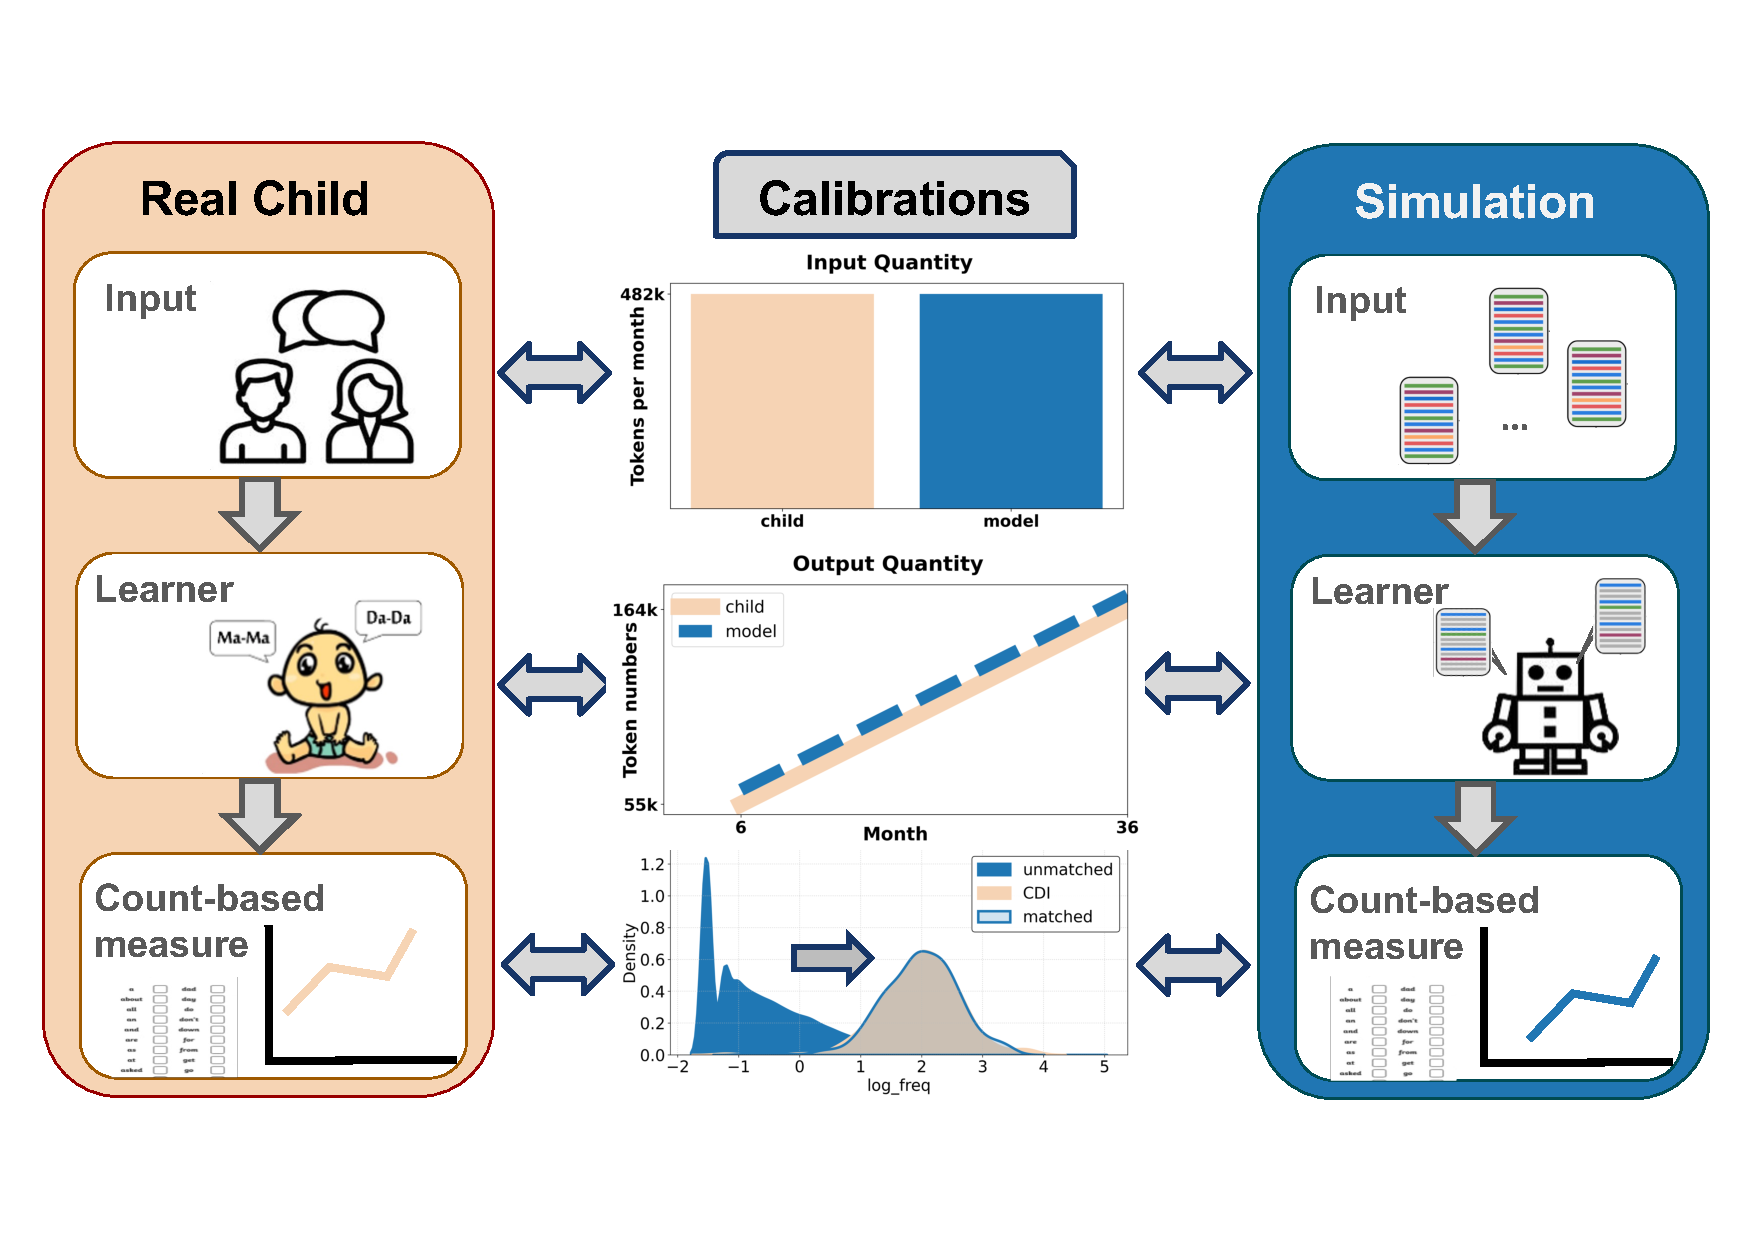
\includegraphics[width=0.5\textwidth]{fig/overview.pdf}}
\caption{\textbf{Overview of the \meCDI{} benchmark framework.} (a) Training and generation sizes are aligned with age-appropriate estimates of linguistic exposure and production from 6–36 months \citep{cristia2019child}. (b) Evaluation sets match the frequency distribution of MacArthur–Bates CDI words in child-directed speech (English-CHILDES).}
\label{fig:overview}
\end{figure}


\subsection{\meCDI{} Benchmark Overview}

The \meCDI{} benchmark enables direct comparison between language model generation and child production through three methodological calibrations to address common mismatches in prior work (Figure~\ref{fig:overview}):


\noindent\textbf{(1) Age-appropriate training exposure:} Training sets are scaled to match cumulative linguistic input from 6–36 months of age estimated from daylong recordings \citep{cristia2019child}.

\noindent\textbf{(2) Production quantity matching:} Generation sizes are calibrated to children's monthly word production rates estimated from longitudinal corpora \citep{cristia2019child} to ensure comparable sample sizes for vocabulary assessment.


\noindent\textbf{(3) Frequency-matched evaluation words:} The evaluation vocabulary is drawn from the MacArthur–Bates Communicative Development Inventory \citep{fenson2007macarthur} and frequency matched to words in English CHILDES corpora.  

We evaluate models on three dimensions: \textit{lexical diversity} (type–token ratio), \textit{word form accuracy} (non-word rate), and \textit{expressive vocabulary size} (\meCDI{} score).


\subsection{Training Data}

We construct two training corpora representing different linguistic environments:

\noindent\textbf{Audiobook corpus:} English audiobook transcripts from LibriVox \citep{kearns2014librivox}, representing narrative-rich, syntactically complex adult-directed language. \noindent\textbf{Child-directed speech (CDS) corpus:} English CHILDES transcripts \citep{macwhinney2000childes}, representing the naturalistic register of early child input.


\paragraph{Age-appropriate scaling} Following \citet{cristia2019child}, we estimate exposure from 250 hours at 6 months to 1,500 hours at 36 months of age. This corresponds to approximately 500 hours of speech input per year, representing a mid-range estimate of children's linguistic environments. Converting speech hours to words using a standard rate of 3 words per second yields training sets ranging from 2.89M words (6 months) to 17.35M words (36 months). Developmental datasets are constructed every 6 months by randomly sampling the target quantity from each corpus (see Table~\ref{tab:train}). Given English CHILDES contains a total of 15.6M words of caregiver inputs, the available data is equivalent to those at the 30-month level, which thus serves as the maximum training input. We emphasize that this scaling controls for \emph{total input quantity} rather than assuming uniform structure of children’s linguistic environments across months.



\paragraph{Preprocessing} All text is lowercased, with spaces and basic punctuation (periods, commas, apostrophes) preserved as word boundary markers. No tokenization or subword segmentation is applied, forcing models to infer word boundaries directly from raw character sequences.

\subsection{Model Architectures and Training}

We train character-level autoregressive models under two architectures: \textbf{LSTM} Three layers with 200-dimensional character embeddings, 1024-dimensional hidden states, and 200-dimensional output projections, following \citet{lavechin2023babyslm}. \textbf{Transformer} GPT-2-style decoder-only architecture with 12 transformer layers, 512-dimensional hidden states, 12 attention heads per layer, following \citet{goriely2024babble}. 


\paragraph{Training procedure} Models are trained to minimize cross-entropy loss using the Adam optimizer (learning rate 0.0001, $\beta_1=0.9$, $\beta_2=0.98$) with inverse square root learning rate decay and 10,000 warmup steps. We train until validation perplexity converges. For each age-corpus pair, two models are trained with same random seeds and non-overlapping data subsets. Training details are provided in Table~\ref{tab:model}.


\paragraph{Generation procedure} At inference time, we generate text using temperature sampling with $T \in \{0.3, 0.6, 1.0, 1.5\}$. Generation begins with a beginning-of-sequence (BOS) token and continues until reaching the target word count corresponding to children's estimated monthly production at that developmental stage (see Table~\ref{tab:speech-metrics} in Appendix). Character sequences are segmented into words using space and punctuation boundaries. For months 31–36, outputs are generated from the same model checkpoints. Because the CDS corpus contains a total of 15.6M words of caregiver input, this limits the age-appropriate training to the 30-month equivalent. For months 31–36, we generate outputs using the same 30-month checkpoint, scaling generation lengths according to children’s estimated production, while noting that the training exposure does not increase beyond 30 months. This ensures a consistent comparison across developmental stages while respecting the corpus limitations.


\subsection{Evaluation Set Construction} \label{sec:eval_construction}
\paragraph{Base vocabulary and POS filtering} We start with the MacArthur-Bates Communicative Development Inventory (CDI) \citep{fenson2007macarthur}, a standardized checklist of 680 English words with normative age-of-production data. To control for lexical class effects, we apply POS tagging using a RoBERTa-based SpaCy pipeline. For each word, POS labels are aggregated across contexts and majority voting is applied separately in each corpus. Function words (articles, pronouns, prepositions, auxiliaries) are excluded, retaining nouns, verbs, adjectives, and adverbs.

\paragraph{Frequency stratification} Filtered CDI words are divided into six frequency bands based on their occurrence in child-directed speech (adult input in English CHILDES), with an equal number of words per band. 

\paragraph{Audiobook subset selection}

For a comparable evaluation, we construct a matched audiobook subset using the same POS filtering and frequency banding. Words are selected such that their frequency distribution mirrors the filtered CDI evaluation set. This process yields two aligned datasets: i.) Filtered CDI evaluation set with 420 words in six frequency bands; and ii.) frequency-matched audiobook subset with the same size per frequency band. This enables a developmentally grounded comparison between model generations and children’s expressive vocabulary.



\subsection{Evaluation Metrics}

We assess model performance using three complementary metrics capturing lexical diversity, form accuracy, and expressive vocabulary.


\paragraph{Type-Token Ratio (TTR)} Measures lexical diversity as the ratio of unique word types to total word tokens. Following \citet{rasanen2024age}, we compute TTR over fixed-size chunks of 3,500 words to control for sample size effects, then average across all chunks.

\paragraph{Non-word Rate} Quantifies word form accuracy as the proportion of generated word types not found in comprehensive English dictionaries: CELEX \citep{van2014subtlex}, the Enchant library,\footnote{\url{https://pypi.org/project/pyenchant/}} and Wiktionary.\footnote{\url{https://www.wiktionary.org}} A word is classified as valid if it appears in any of these three resources. This metric captures models' ability to produce orthographically valid English words.


\paragraph{\meCDI{} Score} Adapts the human CDI vocabulary assessment to model generations through a count-based criterion. We mark a word as "known" if it appears at least $\tau$ times in the generated sample. To determine $\tau$, we analyze CHILDES child productions and fit the resulting vocabulary growth curve to the empirical CDI trajectory. We select $\tau = 60$, which yields slopes most consistent with observed developmental patterns. The \meCDI{} score is computed as:
$$
\text{CDI} = \frac{|\{w \in \text{eval set} : \text{count}(w) \geq \tau\}|}{|\text{eval set}|}
$$
where the evaluation set includes 420 words. This value represents the proportion of age-appropriate vocabulary that the model generates with sufficient frequency to be considered "known." Sensitivity analyses for alternative thresholds ($\tau \in \{1, 500\}$) are shown in Figure~\ref{fig:threshold}.





\section{Results}

\begin{figure*}[!htp]
\centering
\subfloat{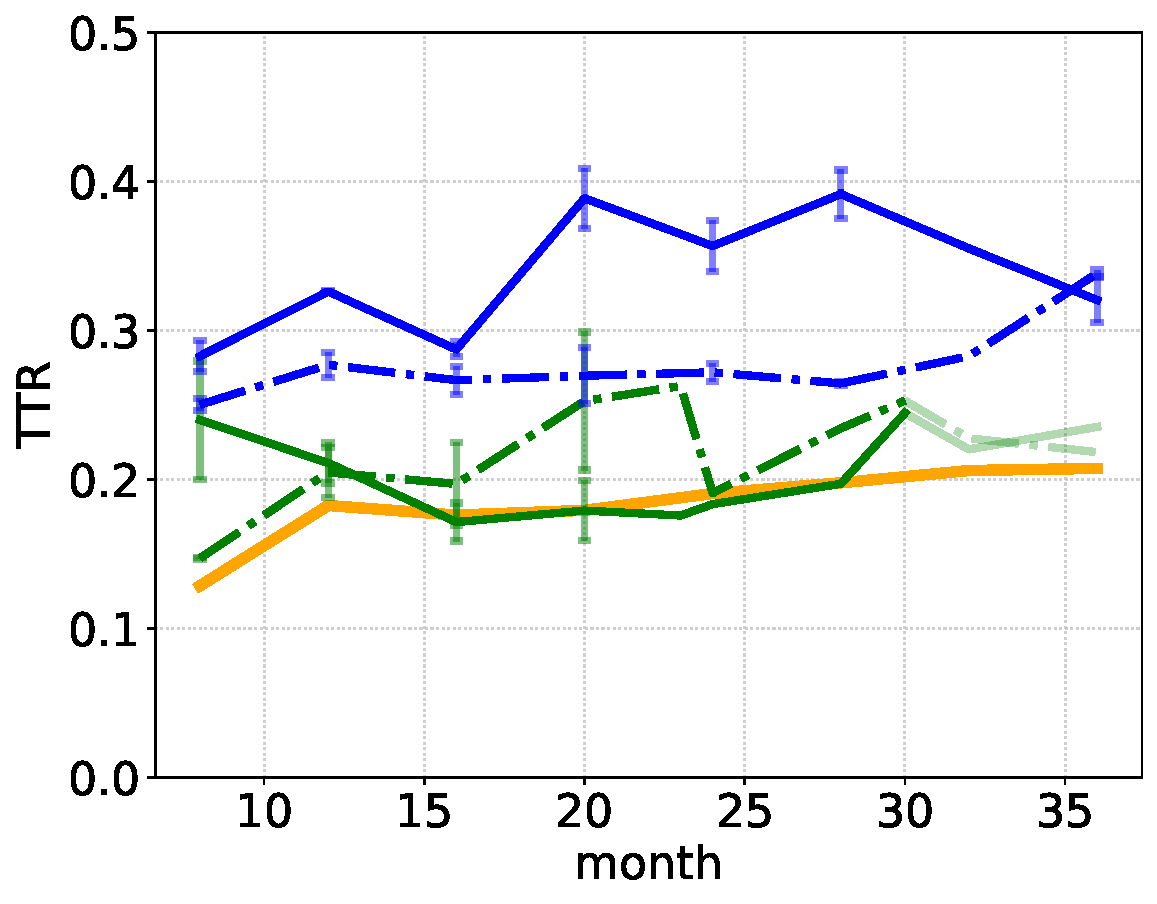
\includegraphics[width=0.27\textwidth]{fig/ttr_500_1.pdf}}
\hspace{2pt}
\subfloat{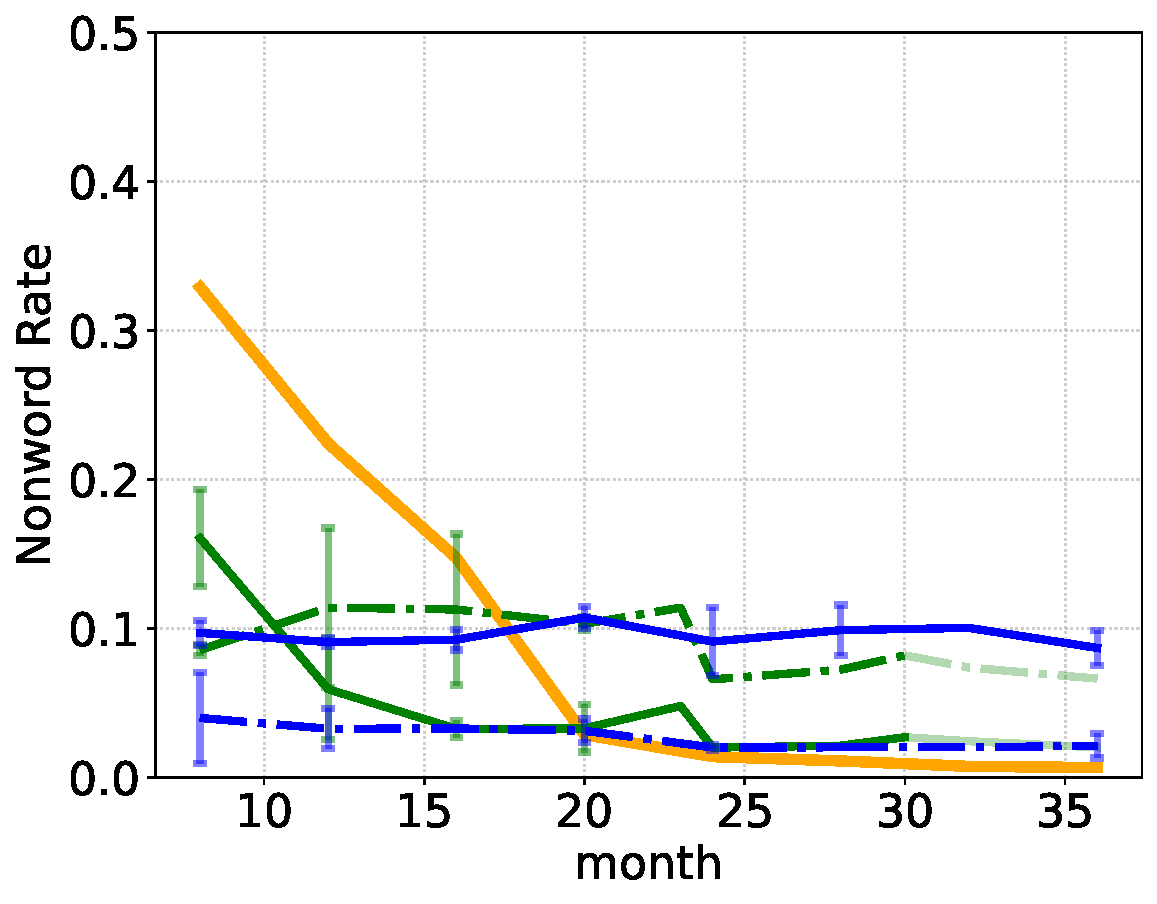
\includegraphics[width=0.27\textwidth]{fig/Nonword Rate_500_1.pdf}}
\hspace{2pt}
\subfloat{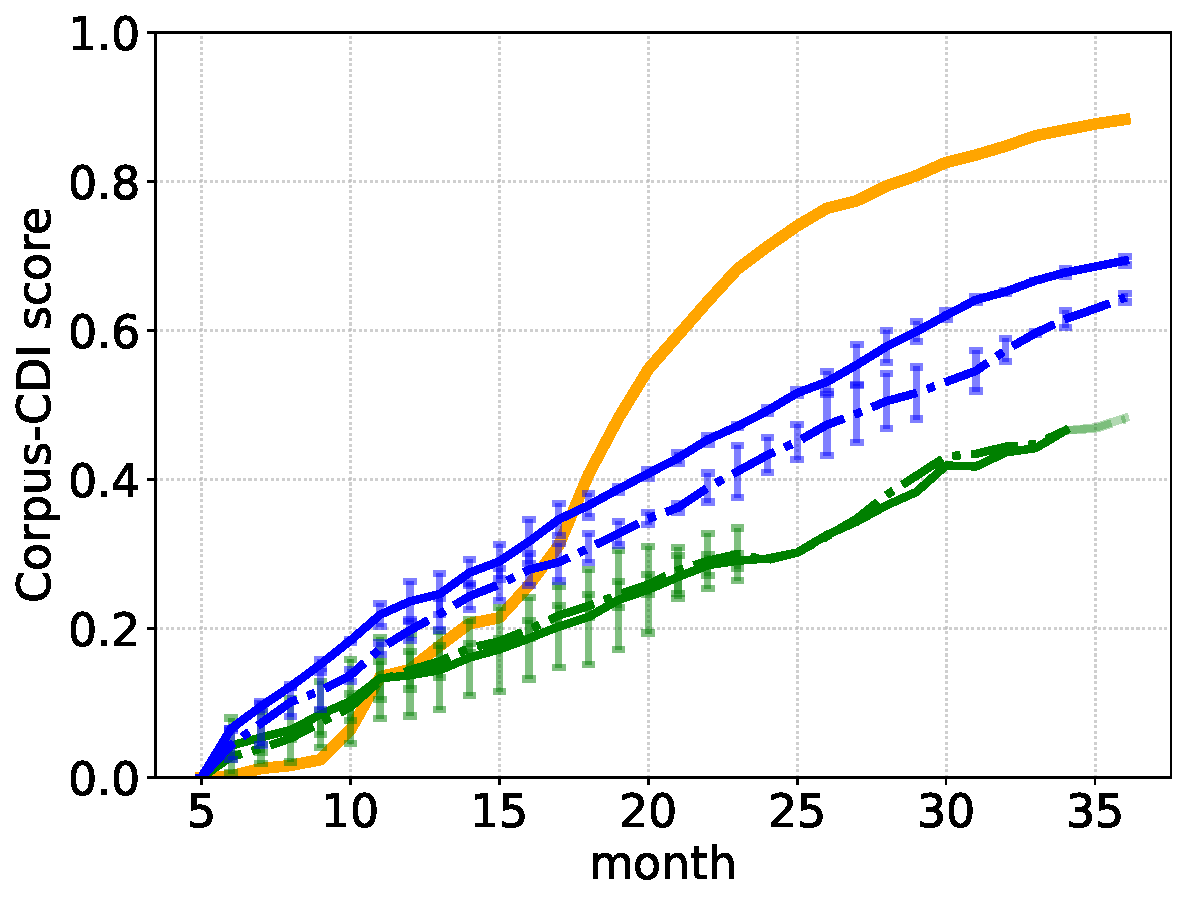
\includegraphics[width=0.27\textwidth]{fig/Corpus-CDI score_500_1.pdf}}
\hspace{2pt}
\subfloat{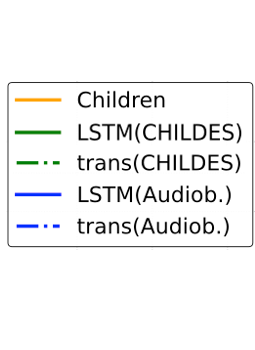
\includegraphics[width=0.13\textwidth]{fig/legend.png}}
\caption{\textbf{Core metrics comparing child and model vocabulary development across age groups.} Left: Type–token ratio (TTR) measuring lexical diversity. Middle: Non-word type rate indicating the proportion of invalid word forms. Right: \meCDI{} scores tracking vocabulary acquisition (words counted as known if produced $>$60 times). Results are shown for LSTM and Transformer models trained on audiobooks and child-directed speech (CDS), compared with CHILDES child production data. Error bars denote 95\% confidence intervals across disjoint training subsets. For the final months (32–36), outputs are generated from the same model checkpoint and shown with lighter transparency.}
\label{fig:core_metric}
\end{figure*}





\begin{figure*}[!ht]
\centering
\subfloat{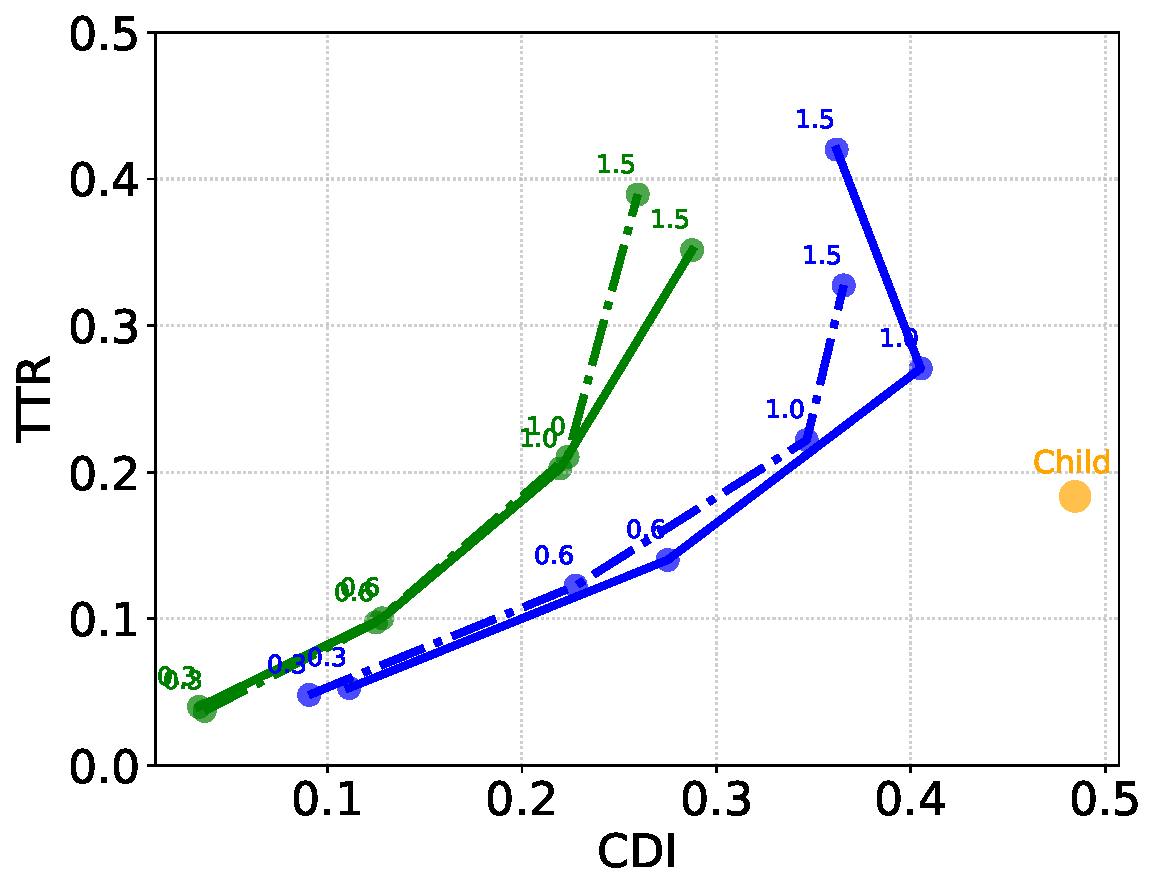
\includegraphics[width=0.35\textwidth]{fig/temp_ttr_500_1.pdf}}
\hspace{2pt}
\subfloat{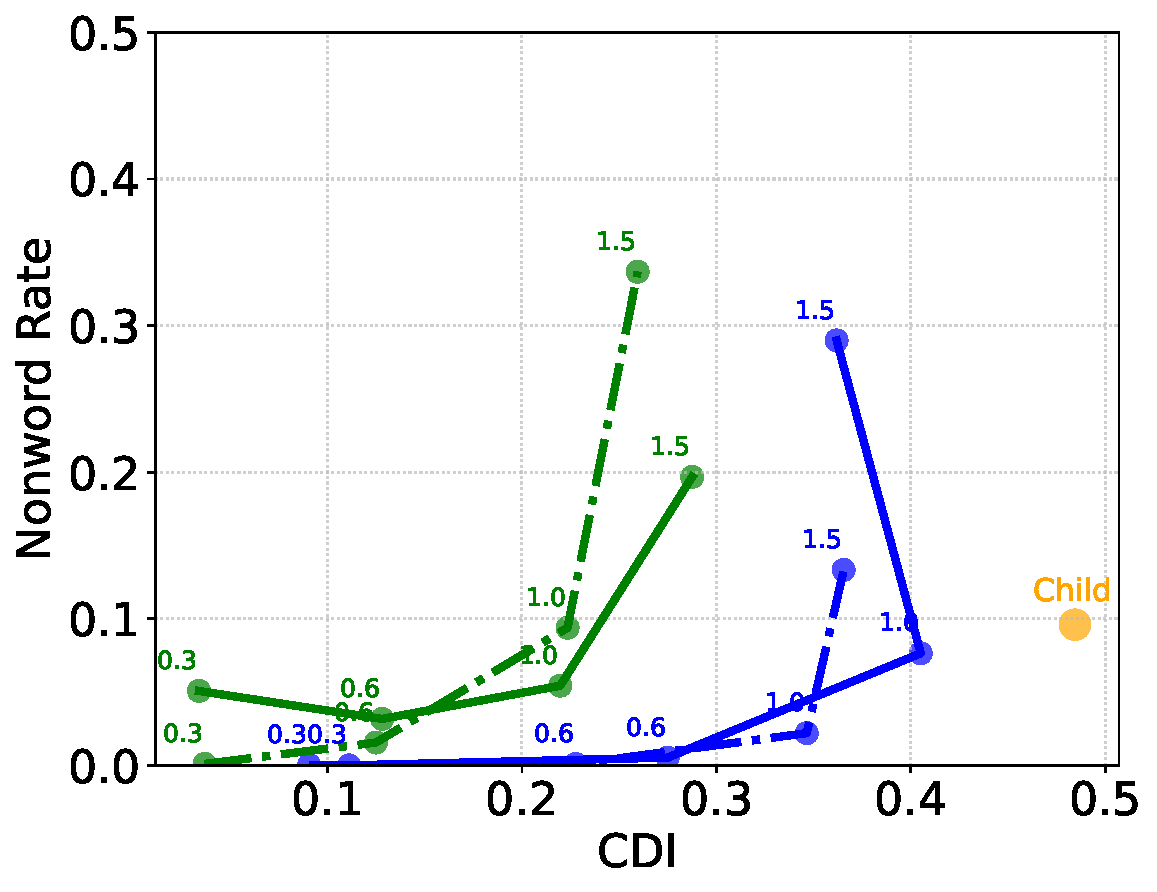
\includegraphics[width=0.35\textwidth]{fig/temp_Nonword Rate_500_1.pdf}}
\hspace{2pt}
\hspace{2pt}
\subfloat{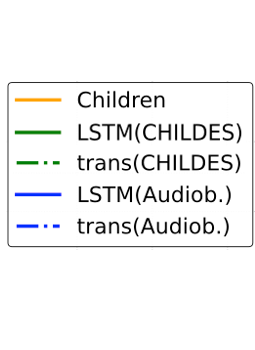
\includegraphics[width=0.13\textwidth]{fig/legend.png}}
\caption{\textbf{Temperature trade-off across different metrics; temperature settings (0.3-1.5)} Left: Trade-off between type-token ratio and CDI score. Right: Relationship between non-word rate and CDI score.  Points show mean scores across models, with numbers illustrating temperature values.}
\label{fig:temp_effect}
\end{figure*}





 
\subsection{Developmental Trajectories}
\label{sec:trajectories}

Figure~\ref{fig:core_metric} presents model performance across three complementary metrics as a function of cumulative training exposure (6-36 months), compared against children's developmental trajectories from CHILDES production data. All results use temperature $T=1.0$ as the default setting.

\paragraph{Lexical diversity} Both LSTM and Transformer models exhibit higher type-token ratios (TTR) than children across developmental stages. Models trained on audiobooks show slightly higher TTR than those trained on child-directed speech, reflecting broader lexical variety in narrative text. Unlike children, whose TTR gradually increases with age, model TTR remains relatively stable. This suggests models generate more lexically diverse outputs from early on, but does not increase substantially with additional training data.


\paragraph{Word form accuracy} Models and children show different developmental patterns in non-word production rates. Children begin with high non-word rates that decrease sharply by the 24th month, reflecting the gradual development of articulatory control and phonological mastery. In contrast, both model architectures maintain relatively stable non-word rates across all training quantities, showing minimal improvement with increased data exposure. Transformers produce slightly fewer non-words than LSTMs, but neither captures the steep improvement observed in children. This divergence likely reflects a critical limitation of text-based models: they cannot capture the development of articulatory-motor control that drives children's decreasing error rates. 



\paragraph{Vocabulary growth} \meCDI{} scores show that children's vocabulary grows sigmoidally, with rapid acceleration during the vocabulary spurt. Models, by contrast, display roughly linear growth, with Transformers slightly outperforming LSTMs and audiobook-trained models outperforming CDS-trained ones. Critically, neither architecture reproduces the accelerating trajectory characteristic of human vocabulary development even as training data accumulates as the estimated quantity.

Across all three metrics, models exhibit qualitatively different developmental patterns from children. They show excessive lexical diversity, minimal improvement in word form accuracy, and slower vocabulary growth that lacks the characteristic acceleration of human development. These differences persist across both architectures and training corpora, suggesting they reflect fundamental limitations in how current language models learn from sequential exposure rather than artifacts of specific model choices. In the following sections, we investigate two potential explanations for these gaps: whether alternative temperature settings during decoding can better align model behavior with children (Section~\ref{sec:temperature}), and whether the observed differences relate to models' frequency-dependent learning patterns (Section~\ref{sec:frequency}).


\subsection{Temperature Tradeoff} 
\label{sec:temperature}

The developmental gaps observed in Section~\ref{sec:trajectories} raise an important question: could these differences arise from suboptimal generation parameters rather than inherent learning limitations? Temperature sampling controls generation stochasticity, with lower temperatures favoring high-probability outputs and higher temperatures increasing diversity. We evaluate whether any temperature setting can align models with children across all three metrics.

Figure~\ref{fig:temp_effect} shows the relationships between metrics as temperature varies from 0.3 to 1.5. Each point represents the mean performance across all developmental stages for a given architecture, corpus, and temperature combination.

\paragraph{TTR-CDI trade-off} Models exhibit a clear trade-off: increasing temperature simultaneously raises type-token ratio (TTR) and \meCDI{} scores. Low temperatures produce TTR values closer to children’s range but severely underrepresent vocabulary size, whereas high temperatures improve vocabulary coverage at the cost of excessive lexical diversity. No temperature setting positions models within the child-like range for both metrics. Audiobook-trained models consistently overshoot children’s TTR, while CDS-trained models come closer but still fall short in vocabulary size. This indicates that the repetitive, high-frequency vocabulary characteristic of early child speech cannot be recovered through decoding adjustments alone. 


\paragraph{Non-word-CDI trade-off} Higher temperatures increase non-word rates for both architectures. While some CDS-trained models at intermediate temperatures approximate children’s average non-word rates, this alignment is misleading: children’s non-word rates decrease sharply over development, whereas models remain largely static. Moreover, achieving this partial alignment comes at the expense of TTR matching, suggesting that it is still implausible to simultaneously satisfy multiple developmental constraints.


These results demonstrate that temperature tuning cannot resolve the developmental misalignment between models and children. The gaps reflect fundamental differences in how models and children balance vocabulary size, lexical diversity, and production accuracy. Post-hoc decoding adjustments cannot substitute for differences in underlying learning and production mechanisms. In the next section, we examine whether these differences relate to frequency-dependent learning patterns.



\subsection{Frequency effect} 
\label{sec:frequency}

\begin{figure}[!h]
\centering
\adjustbox{trim={30 20 30 20}, clip}{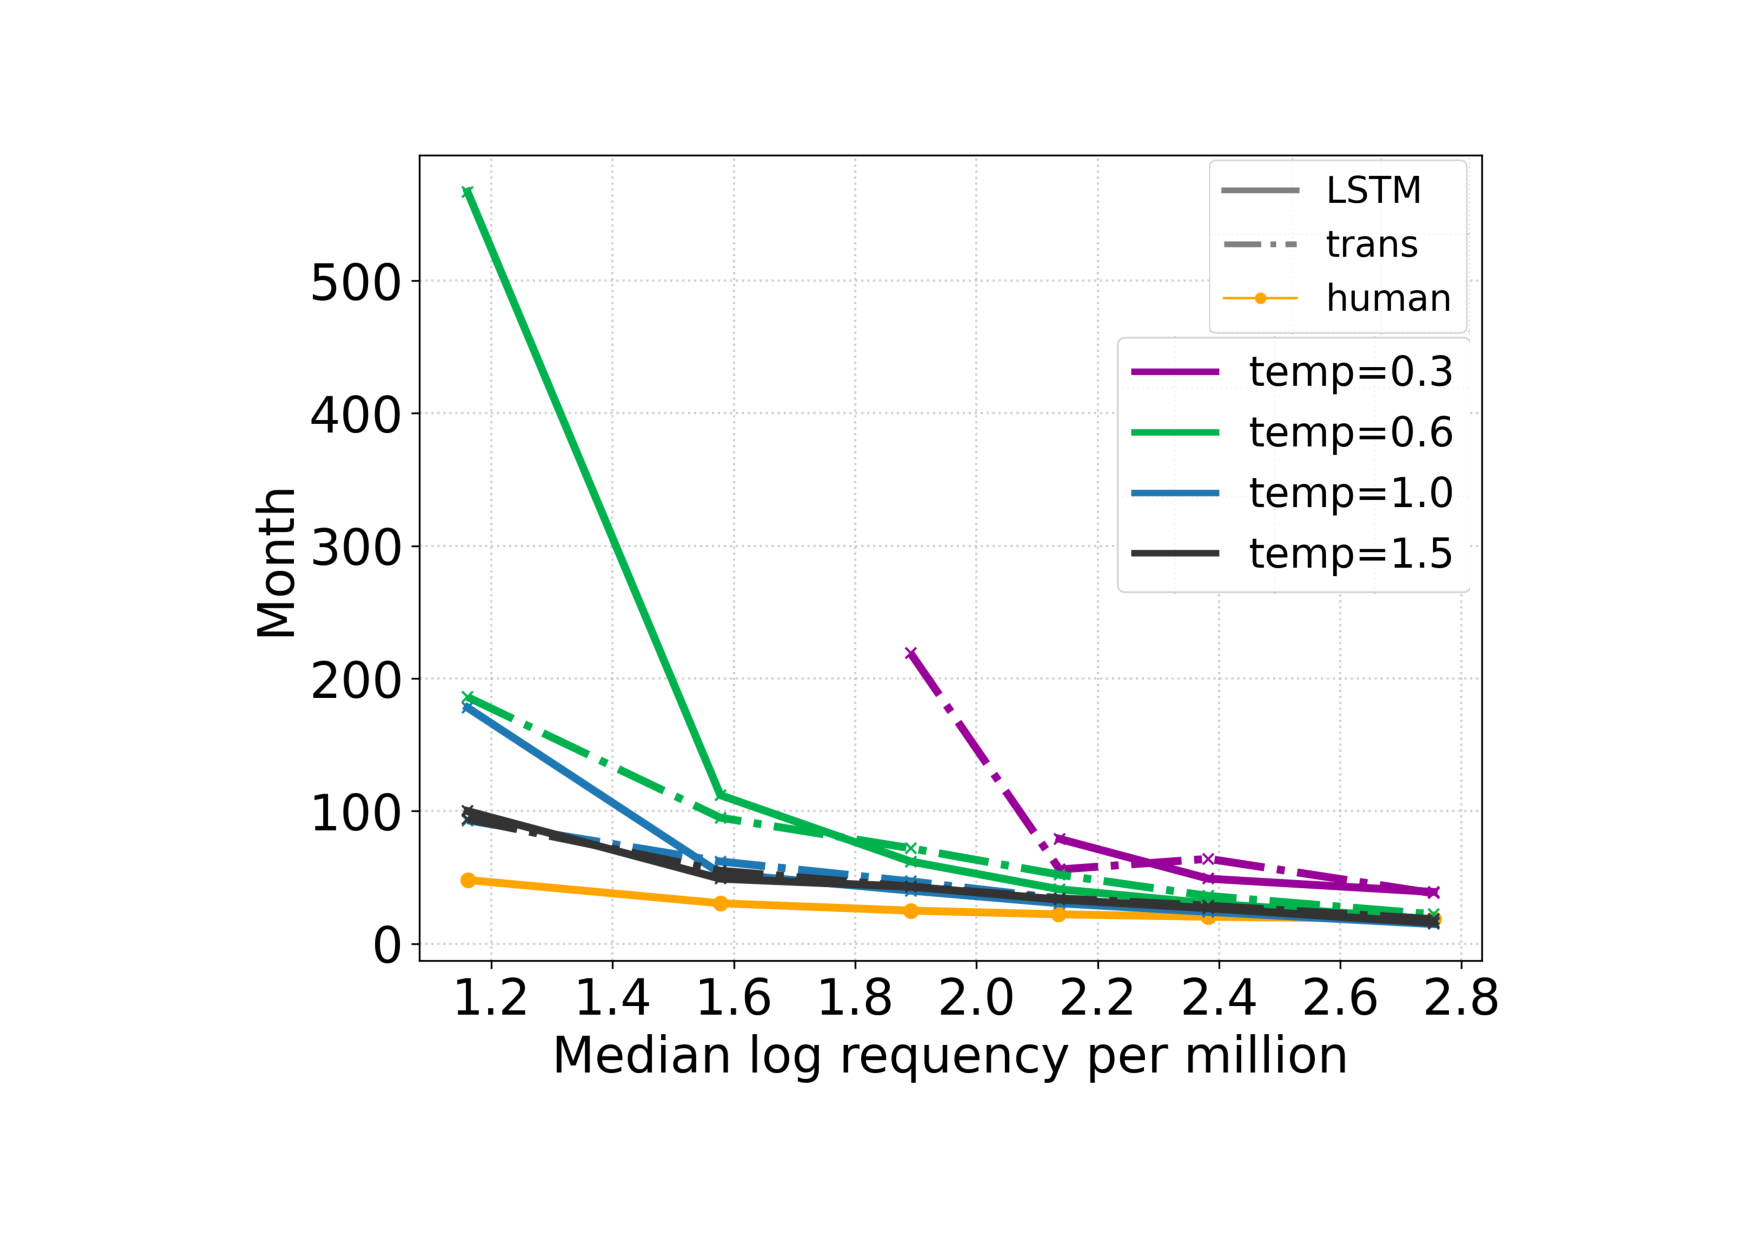
\includegraphics[width=0.6\textwidth]{fig/freq_stela.pdf}}
\caption{\textbf{Extrapolated months across different datasets for models trained on audiobooks}. x-axis: log frequency per million in training data; y-axis:estimated developmental month at which models reach 80\% mastery for each frequency band. Missing points of the lower frequency bands of temperature =0.3 come from 0 }
\label{fig:freq_effect}
\end{figure}


The analyses so far show that models lag far behind children in vocabulary acquisition, and this gap cannot be closed by tuning generation parameters. We now ask whether this delay is uniform across input frequency. To test this, we divided the vocabulary into six frequency bands based on child-directed speech and tracked the proportion of words acquired in each band, using the same sigmoid growth curve fitting as above. For each band, we extracted the \textit{extrapolated age of acquisition}, defined as the cumulative training exposure at which the model reaches 80\% mastery, matching the maximum rate observed in CDI norms. This “months-to-mastery” measure quantifies how quickly different frequency bands are learned as a function of cumulative training exposure.


\paragraph{Divergent frequency sensitivity} Figure~\ref{fig:freq_effect} shows that children show much weaker frequency dependence than models, with only modest variation between high- and low-frequency vocabulary. By contrast, both models display considerable frequency dependence: high-frequency words are acquired relatively quickly, but acquisition times for low-frequency words increase by orders of magnitude. This indicates that models rely heavily on repeated exposure, whereas children generalize more effectively from sparse input.


\paragraph{Temperature modulation} Temperature settings systematically modulate frequency effects. At low temperatures ($T=0.3$), models fail to acquire rare words, as deterministic decoding prevents them from being generated sufficient times to count as "known". Higher temperatures ($T=1.0$–$1.5$) alleviate this issue by surfacing rare words more often, but the improvement remains limited: even under the most favorable conditions, models require many times more exposure than children to acquire low-frequency vocabulary. Thus, temperature affects severity of the bias but not the underlying cause.


\paragraph{Long-tail truncation} These results point to long-tail truncation as the primary mechanism underlying models' vocabulary acquisition gap. Language models are trained to minimize cross-entropy loss, which optimizes for predicting the most probable next character given context. This objective inherently prioritizes frequent patterns: prediction errors on common words contribute more to loss than on rare words, leading models to allocate representational capacity proportionally to frequency. 


Children, by contrast, do not optimize for predictive accuracy. Their learning mechanisms such as explicit memory for individual word-learning episodes \citep{markson1997evidence}, cross-situational inference\citep{smith2008infants}, and social-pragmatic cues \citep{tomasello2000social} allow them to acquire words from sparse observations without requiring proportional exposure. This qualitative difference in learning objective, rather than mere data inefficiency, explains why children succeed in the long tail where models consistently fail.


\subsection{Production of Content Words}
\label{sec:content_word}


\begin{figure}[!h]
\centering
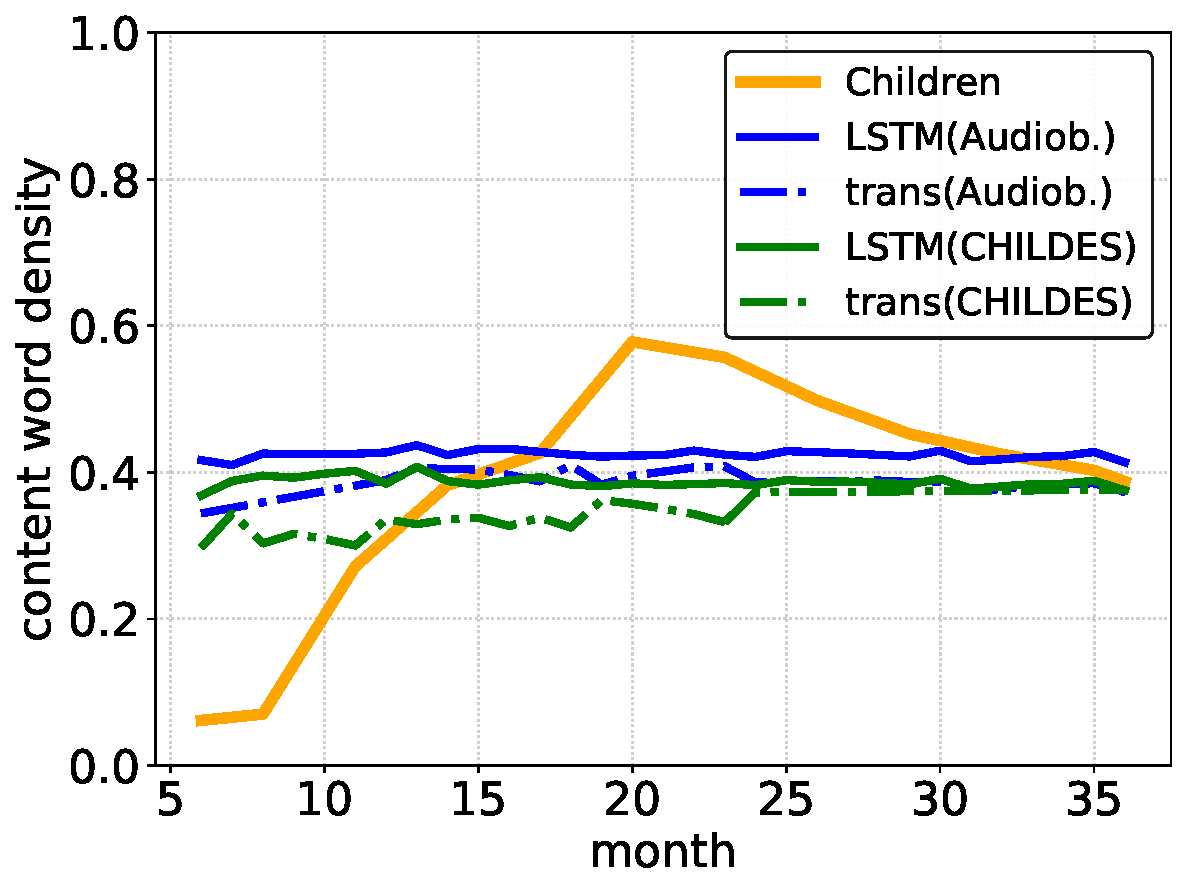
\includegraphics[width=0.48\textwidth]{fig/content_500_1.pdf}
\caption{\textbf{Proportion of content words in generated text across development.} Children show an inverse U-shaped trajectory, while all model configurations maintain stable proportions around 40\% across training stages.}
\label{fig:content_prop}
\end{figure}


The frequency-dependent learning patterns in Section~\ref{sec:frequency} may partly stem from differences in functional versus content word production. Function words dominate the highest-frequency bands \citep{zipf2016human}, whereas our \meCDI{} evaluation targets content words (Section~\ref{sec:eval_construction}). Over-reliance on function words could explain why models achieve lower CDI scores and limited lexical diversity: frequent repetition of a small set of functional items increases token counts without expanding the number of unique word types.


\paragraph{Children’s inverse U-shaped trajectory} Figure~\ref{fig:content_prop} shows that children exhibit a pronounced inverse U-shaped trajectory in content word production. Early productions contain few content words, followed by a sharp rise during the vocabulary spurt, and then a decline as grammatical function words become integrated \citep{bates1994developmental,brown1973first}. Critically, this declining phase coincides with children's steepest \meCDI{} growth (Figure~\ref{fig:core_metric}), showing that children’s vocabulary growth is not simply driven by frequency exposure but by a qualitative reorganization of their lexical production.

\paragraph{Models’ invariant balance} 

In contrast, all model configurations maintain stable content-word proportions around 40\%, which closely matches adult English distributions \citep{biber2021grammar}. This invariance holds across architectures and training corpora: both CDS- and audiobook-trained models converge almost immediately to corpus-level statistics and remain fixed throughout training.

This invariance helps explain several earlier findings: (1) Frequency truncation (Section~\ref{sec:frequency}) disproportionately harms content words, which spread more evenly across frequency bands. (2) CDI underperformance reflects systematic undergeneration of content words, on which CDI norms are based. (3) Elevated TTR may paradoxically arise from over-allocating tokens to a small set of high-frequency function words, forcing broader but shallower sampling of content vocabulary.

Taken together, these results reveal a fundamental mismatch: cross-entropy training aligns models with corpus-level statistics but not with children’s developmental trajectory. While children dynamically restructure their lexicon and functional–content balance, models remain tied to static frequency distributions.



\section{Discussion}

We introduced \meCDI{}, a benchmark that enables direct comparison between children’s expressive vocabulary and language model generations by aligning training exposure, production quantity, and frequency distributions. Our analyses yield three main findings that highlight key differences between human and model vocabulary acquisition.


First, while both character-level LSTMs and Transformers expand their vocabularies with increased training data, their developmental trajectories diverge largely from those of children. Models consistently produce far greater lexical diversity, maintain stable non-word rates across training, and exhibit slower vocabulary growth without the characteristic acceleration observed in children. These patterns generalize across architectures (LSTM vs. Transformer) and training corpora (audiobooks vs. child-directed speech), suggesting that the underlying learning mechanisms driving word acquisition differ fundamentally between children and current language models. In other words, the mismatch is not tied to the choice of corpus or model architecture, but reflects mechanistic differences in how children versus models acquire and prioritize vocabulary.


Second, these divergences cannot be reconciled through parameter tuning at generation time. Temperature variation experiments show that no single setting simultaneously aligns models with children across TTR, non-word rate, and vocabulary size. The gap thus arises from fundamental properties of the learning and production mechanisms rather than from suboptimal decoding choices.


Third, frequency analyses reveal the mechanistic source of these differences. Children acquire words across frequency bands within a narrow age window (around 35–40 months), whereas models require exponentially more exposure for low-frequency words (equivalent to 300–600 months of input for words around log frequency 1.2–1.4 per million). This extreme frequency sensitivity follows directly from cross-entropy optimization, which down-weights rare words during training. Importantly, the interaction with word categories amplifies the divergence: models preserve adult-like content/function ratios (around 40\% content words) throughout training, while children show a U-shaped trajectory driven by the integration of function words. Since function words cluster in high-frequency bands whereas content words (the CDI evaluation focus) distribute more evenly, models' frequency-proportional learning underproduces the vocabulary class children prioritize.


These findings point to limitations of predictive accuracy as the sole training objective for modeling acquisition. Children do not rely solely on distributional statistics; they integrate referential grounding, social-pragmatic inference, and episodic memory of word-learning events to acquire vocabulary from sparse observations. Progress in cognitively grounded language modeling may therefore require learning objectives beyond predictive accuracy, such as memory-augmented architectures for rare word retention, contrastive objectives that emphasize lexical representations, or interactive learning paradigms where production influences subsequent input.


 
\section{Limitations}

Our evaluation framework has several limitations. First, we evaluate character-level models rather than speech-based systems. While character input provides an upper bound by preserving invariant word forms and explicit boundaries, it bypasses the acoustic variability and segmentation challenges that infants solve \citep{dupoux2018cognitive}. Speech-based language models \citep{lakhotia2021generative,nguyen2024spirit} must additionally contend with phonetic variability and ambiguous word boundaries. As such, our reported gaps likely underestimate the difficulty of vocabulary acquisition in more realistic, speech-based models. Extending \meCDI{} to speech therefore requires addressing the non-trivial task of mapping continuous acoustic output into discrete word forms suitable for CDI scoring and we would expect even larger divergences from children's developmental trajectories. Moreover, our models lack multimodal grounding—the word-object associations and interactive feedback that children exploit. Such grounding likely supports children’s frequency-independent learning by providing alternative cues beyond distributional statistics.

Second, the CHILDES transcripts used as reference data introduce possible biases. Transcribers often normalize children’s productions by correcting errors or completing fragments, which may underestimate non-word rates and inflate apparent model–child gaps. Conversely, our character-level models inherently generate orthographically valid forms, potentially overstating their production accuracy relative to children’s speech.


Third, our comparison of parental CDI reports with model outputs involves methodological misalignment. CDI scores reflect whether parents judge a child to “say” a word, capturing semantic knowledge and contextual usage in addition to production capability. In contrast, our \meCDI{} metric counts raw production frequency in unconstrained model text. A child uttering dog once demonstrates robust lexical knowledge, whereas a model generating dog 60 times may not. While our threshold ($\tau = 60$) calibrates vocabulary growth slopes, the construct validity gap between CDI reports and model generation remains.


Finally, our study focuses on English and a single vocabulary assessment tool (CDI). Cross-linguistic validation is essential for establishing universality: languages with richer morphology, less transparent orthography, or different child-directed registers may yield different alignments between model and child learning. Character-level models in particular may be sensitive to orthographic properties, limiting generalizability beyond English.


\section{Ethics Statement}

All data used in this study are publicly available through the CHILDES database. Our work focuses exclusively on model benchmarking and internal simulations, with the goal of advancing fundamental research on language acquisition. We emphasize that the evaluations conducted here are not sufficient for deployment in real-world applications. Any future use involving human data should undergo rigorous validation and appropriate de-identification procedures to ensure privacy and ethical compliance.



% \section*{Acknowledgments}
% add erc affiliations from the template

% Bibliography entries for the entire Anthology, followed by custom entries
%\bibliography{anthology,custom}
% Custom bibliography entries only
%\newpage

\newpage

\section{Appendix}

\subsection{Training and generation details}

Table~\ref{tab:train} summarizes the age-appropriate scaling of training data across three exposure scenarios. Linguistic exposure estimates are based on daylong recording studies \citep{cristia2019child}, which document substantial variability in the amount of speech heard by children across environments. Annual exposure ranges from approximately 100 hours in low-input households to 1000 hours in high-input ones, with 500 hours per year representing a mid-range estimate.

Cumulative exposure thus increases from 50–500 hours at 6 months to 300–3000 hours by 36 months. Assuming a standard speech rate of three words per second, this corresponds to training sets ranging from 0.58M words (6 months, low exposure) to 34.71M words (36 months, high exposure).


\begin{table}[ht]
\centering
\small
\begin{tabular}{l c c c c}
\toprule
\textbf{Age} & \textbf{Hours} & \textbf{Words} & \textbf{Characters} & \textbf{Utterances} \\

\midrule
\multicolumn{5}{l}{\textit{Low exposure scenario (100 hours/year)}} \\
\midrule
6   & 50   & 0.58  & 2.95  & 58   \\
12  & 100  & 1.16  & 5.89  & 116  \\
18  & 150  & 1.73  & 8.84  & 173  \\
24  & 200  & 2.31  & 11.78 & 231  \\
30  & 250  & 2.89  & 14.73 & 289  \\
36  & 300  & 3.47  & 17.67 & 347  \\
\midrule
\multicolumn{5}{l}{\textit{Medium exposure scenario (500 hours/year)}} \\
\midrule
6   & 250  & 2.89  & 14.73 & 289  \\
12  & 500  & 5.78  & 29.45 & 578  \\
18  & 750  & 8.68  & 44.18 & 868  \\
24  & 1000 & 11.57 & 58.90 & 1157 \\
30  & 1250 & 14.46 & 73.63 & 1446 \\
36  & 1500 & 17.35 & 88.35 & 1735 \\
\midrule
\multicolumn{5}{l}{\textit{High exposure scenario (1000 hours/year)}} \\
\midrule
6   & 500  & 5.78  & 29.45 & 578  \\
12  & 1000 & 11.57 & 58.90 & 1157 \\
18  & 1500 & 17.35 & 88.35 & 1735 \\
24  & 2000 & 23.14 & 117.80 & 2314 \\
30  & 2500 & 28.92 & 147.25 & 2892 \\
36  & 3000 & 34.71 & 176.70 & 3471 \\
\bottomrule
\end{tabular}
\caption{\textbf{Age-appropriate scaling of training datasets across three exposure scenarios.} Estimates are derived from three exposure scenarios (100h, 500h, 1000h per year), reflecting observed variability in children’s linguistic environments \citep{cristia2019child}. Word counts assume 3 words/second; character counts assume 5.1 characters/word; utterance counts assume 10 words/utterance.}
\label{tab:train}
\end{table}


Model training employed carefully tuned hyperparameters (Table~\ref{tab:model}), selected through systematic validation experiments to ensure training stability and computational efficiency across different data scales.


\begin{table}[ht]
\centering
\begin{tabular}{@{} l l @{}}
\hline
\textbf{Hyperparameter} & \textbf{Value} \\
\hline
Max sequence length & 1024 \\
Batch size & 64 \\
Learning rate & 0.0001 \\
Learning rate scheduler & inverse sqrt \\
Warmup steps & 10000 \\
Optimizer & Adam \\
Adam-beta1 & 0.9 \\
Adam-beta2 & 0.98 \\
Dropout & 0.1 \\
\hline
\textbf{LSTM hyperparameter} & \textbf{Value} \\
\hline
decoder layers & 3 \\
hidden size & 1024 \\
embedding dimension & 200 \\
\hline
\textbf{Transformer hyperparameter} & \textbf{Value} \\
\hline
Transformer layers & 12 \\
Intermediate hidden size & 512 \\
Attention heads & 12 \\
Attention dropout & 0.05 \\
\hline
\end{tabular}
\caption{\textbf{Language model training hyperparameters.} Configurations balance model capacity, stability, and efficiency across training scales.}
\label{tab:model}
\end{table}


\begin{table}[!h]
\centering
\begin{tabular}{rrrr}
\toprule
\textbf{month} & \textbf{\#sec/hour} & \textbf{estimation} & \textbf{production} \\
\midrule
6 & 61.25 & 55,125 & 782 \\
7 & 65.30 & 58,769 & 1,323 \\
8 & 69.35 & 62,412 & 1,278 \\
9 & 73.40 & 66,056 & 3,964 \\
10 & 77.44 & 69,699 & 627 \\
11 & 81.49 & 73,343 & 1,148 \\
12 & 85.54 & 76,986 & 1,361 \\
13 & 89.59 & 80,630 & 568 \\
14 & 93.64 & 84,273 & 2,720 \\
15 & 97.69 & 87,917 & 13,765 \\
16 & 101.73 & 91,560 & 3,620 \\
17 & 105.78 & 95,204 & 7,589 \\
18 & 109.83 & 98,847 & 15,197 \\
19 & 113.88 & 102,491 & 17,090 \\
20 & 117.93 & 106,134 & 19,912 \\
21 & 121.98 & 109,778 & 33,458 \\
22 & 126.02 & 113,421 & 33,880 \\
23 & 130.07 & 117,065 & 63,738 \\
24 & 134.12 & 120,708 & 191,062 \\
25 & 138.17 & 124,352 & 130,525 \\
26 & 142.22 & 127,995 & 136,195 \\
27 & 146.27 & 131,639 & 148,741 \\
28 & 150.31 & 135,282 & 158,910 \\
29 & 154.36 & 138,926 & 190,263 \\
30 & 158.41 & 142,569 & 195,549 \\
31 & 162.46 & 146,213 & 196,677 \\
32 & 166.51 & 149,856 & 184,024 \\
33 & 170.56 & 153,500 & 185,534 \\
34 & 174.60 & 157,143 & 185,691 \\
35 & 178.65 & 160,787 & 153,515 \\
36 & 182.70 & 164,430 & 299,537 \\
\bottomrule
\end{tabular}
\caption{\textbf{Monthly progression of speech metrics.} Estimated exposure and production rates over developmental time.}
\label{tab:speech-metrics}
\end{table}

The examples in Table~\ref{tab:generation-examples} highlight distinct generation behaviors across datasets and model architectures under a fixed sampling temperature ($T=1.0$). Models trained on child-directed input (Child, CHILDES) tend to produce shorter, phonologically simple, and semantically grounded utterances, resembling early stages of language development. In contrast, audiobook-trained models generate longer, syntactically structured sequences but often lack pragmatic coherence. Comparing architectures, Transformers exhibit more globally consistent syntax and longer dependency spans, while LSTMs display stronger local predictability but higher rates of morphological irregularities. These qualitative patterns align with quantitative trends observed in our lexical and nonword diversity metrics, underscoring how data type and inductive bias jointly shape emergent linguistic structure.

\begin{table}[ht]
\centering
\begin{tabular}{ll}
\hline
\textbf{Setting} & \textbf{Generated Sequences} \\
\hline
\textbf{Child} & dad \\
                & dada \\
                & mommy looked it missed its wheel \\
                & i want my plate for it \\
\hline
\textbf{Audiobook}       & wounded \\
\textbf{(LSTM)}          & for woman says \\
                & no i don't know what i \\
                & fuller over his week scully a \\
\hline
\textbf{Audiobook}  & to \\
\textbf{(Trans)}                     & o he had been \\
                     & and the work of the lord \\
                     & ascend mass of softly rounded head \\
\hline
\textbf{CHILDES}          & can \\
\textbf{(LSTM)}               & bump \\
               & he said I was wondering what \\
               & yeah detfive wroggy on drh aulf \\
\hline
\textbf{CHILDES}          & on \\
\textbf{(Trans)}                   & helsewhere \\
                   & he doesn't like him does he \\
                   & hafta dragged on doh aunty quite \\
\hline
\end{tabular}
\caption{\textbf{Examples of generated sequences.} Samples are drawn from models trained on different datasets and architectures at a sampling temperature of 1.0. The boundary marker is replaced with blank space for readability.}
\label{tab:generation-examples}
\end{table}


\subsection{Result details}

\begin{table*}[t]
\centering
\setlength{\tabcolsep}{3.5pt}
\small
\begin{tabular}{l c c c c c c c c c}
\toprule
\textbf{Dataset}\\\textbf{(Model)} & \textbf{Temp} & \multicolumn{2}{c}{\textbf{TTR (\%)}} & \multicolumn{2}{c}{\textbf{NWType (\%)}} & \multicolumn{2}{c}{\textbf{NWToken (\%)}} & \multicolumn{2}{c}{\textbf{CDI(\%)}} \\
\cmidrule(lr){3-4} \cmidrule(lr){5-6} \cmidrule(lr){7-8} \cmidrule(lr){9-10}
& & \textbf{Mean} & \textbf{Last} & \textbf{Mean} & \textbf{Last} & \textbf{Mean} & \textbf{Last} & \textbf{Mean} & \textbf{Last} \\
\midrule
\textbf{CHILDES} & - & 18.3 & 20.7 & 9.6 & 0.7 & 4.7 & 0.2 & 48.6 & 88.4 \\
\midrule
\multirow{4}{*}{\begin{tabular}[c]{@{}l@{}}\textbf{Audiobook}\\\textbf{(LSTM)}\end{tabular}} 
& \textbf{0.3} & 43.8 [41.3, 46.1] & 44.2 & 13.5 [12.0, 14.8] & 13.8 & 10.4 [9.2, 11.6] & 10.6 & 62.5 [59.2, 65.8] & 63.1 \\
& \textbf{0.6} & 45.9 [43.4, 48.2] & 46.3 & 14.8 [13.3, 16.1] & 15.1 & 11.7 [10.5, 12.9] & 11.9 & 65.2 [61.9, 68.5] & 65.8 \\
& \textbf{1.0} & 48.1 [45.6, 50.4] & 48.5 & 16.4 [14.9, 17.7] & 16.7 & 13.1 [11.9, 14.3] & 13.3 & 68.8 [65.5, 72.1] & 69.4 \\
& \textbf{1.5} & \textbf{50.3} [47.8, 52.6] & \textbf{50.7} & \textbf{18.0} [16.5, 19.3] & \textbf{18.3} & \textbf{14.8} [13.6, 16.0] & \textbf{15.0} & \textbf{71.9} [68.6, 75.2] & \textbf{72.5} \\
\midrule
\multirow{4}{*}{\begin{tabular}[c]{@{}l@{}}\textbf{Audiobook}\\\textbf{(Trans)}\end{tabular}}
& \textbf{0.3} & 44.5 [42.0, 46.8] & 44.9 & 13.8 [12.3, 15.1] & 14.1 & 10.7 [9.5, 11.9] & 10.9 & 63.2 [59.9, 66.5] & 63.8 \\
& \textbf{0.6} & 46.6 [44.1, 48.9] & 47.0 & 15.1 [13.6, 16.4] & 15.4 & 12.0 [10.8, 13.2] & 12.2 & 65.9 [62.6, 69.2] & 66.5 \\
& \textbf{1.0} & 48.8 [46.3, 51.1] & 49.2 & 16.7 [15.2, 18.0] & 17.0 & 13.4 [12.2, 14.6] & 13.6 & 69.5 [66.2, 72.8] & 70.1 \\
& \textbf{1.5} & \textbf{51.0} [48.5, 53.3] & \textbf{51.4} & \textbf{18.3} [16.8, 19.6] & \textbf{18.6} & \textbf{15.1} [13.9, 16.3] & \textbf{15.3} & \textbf{72.6} [69.3, 75.9] & \textbf{73.2} \\
\midrule
\multirow{4}{*}{\begin{tabular}[c]{@{}l@{}}\textbf{CHILDES}\\\textbf{(LSTM)}\end{tabular}} 
& \textbf{0.3} & 43.8 [41.3, 46.1] & 44.2 & 13.5 [12.0, 14.8] & 13.8 & 10.4 [9.2, 11.6] & 10.6 & 62.5 [59.2, 65.8] & 63.1 \\
& \textbf{0.6} & 45.9 [43.4, 48.2] & 46.3 & 14.8 [13.3, 16.1] & 15.1 & 11.7 [10.5, 12.9] & 11.9 & 65.2 [61.9, 68.5] & 65.8 \\
& \textbf{1.0} & 48.1 [45.6, 50.4] & 48.5 & 16.4 [14.9, 17.7] & 16.7 & 13.1 [11.9, 14.3] & 13.3 & 68.8 [65.5, 72.1] & 69.4 \\
& \textbf{1.5} & \textbf{50.3} [47.8, 52.6] & \textbf{50.7} & \textbf{18.0} [16.5, 19.3] & \textbf{18.3} & \textbf{14.8} [13.6, 16.0] & \textbf{15.0} & \textbf{71.9} [68.6, 75.2] & \textbf{72.5} \\
\midrule
\multirow{4}{*}{\begin{tabular}[c]{@{}l@{}}\textbf{CHILDES}\\\textbf{(Trans)}\end{tabular}}
& \textbf{0.3} & 44.5 [42.0, 46.8] & 44.9 & 13.8 [12.3, 15.1] & 14.1 & 10.7 [9.5, 11.9] & 10.9 & 63.2 [59.9, 66.5] & 63.8 \\
& \textbf{0.6} & 46.6 [44.1, 48.9] & 47.0 & 15.1 [13.6, 16.4] & 15.4 & 12.0 [10.8, 13.2] & 12.2 & 65.9 [62.6, 69.2] & 66.5 \\
& \textbf{1.0} & 48.8 [46.3, 51.1] & 49.2 & 16.7 [15.2, 18.0] & 17.0 & 13.4 [12.2, 14.6] & 13.6 & 69.5 [66.2, 72.8] & 70.1 \\
& \textbf{1.5} & \textbf{51.0} [48.5, 53.3] & \textbf{51.4} & \textbf{18.3} [16.8, 19.6] & \textbf{18.6} & \textbf{15.1} [13.9, 16.3] & \textbf{15.3} & \textbf{72.6} [69.3, 75.9] & \textbf{73.2} \\
\bottomrule
\end{tabular}
\caption{Metric scores across different model settings presented in percentages (\%). Mean values are averaged across different months, followed by range across different models. We also reported the score of the 36th month. TTR: Type-token ratio, NWType: Non-word type rate, NWToken: Non-word token rate. CHILDES child production. Best scores for each setting are in \textbf{bold}.}
\label{tab:temp_metric}
\end{table*}

To establish reliable vocabulary acquisition metrics, we conducted systematic analyses of different word count thresholds (Figure~\ref{fig:threshold}). This calibration process aimed to align our \meCDI{} scores with empirical observations of child vocabulary development.


\begin{figure}[!ht]
\centering
{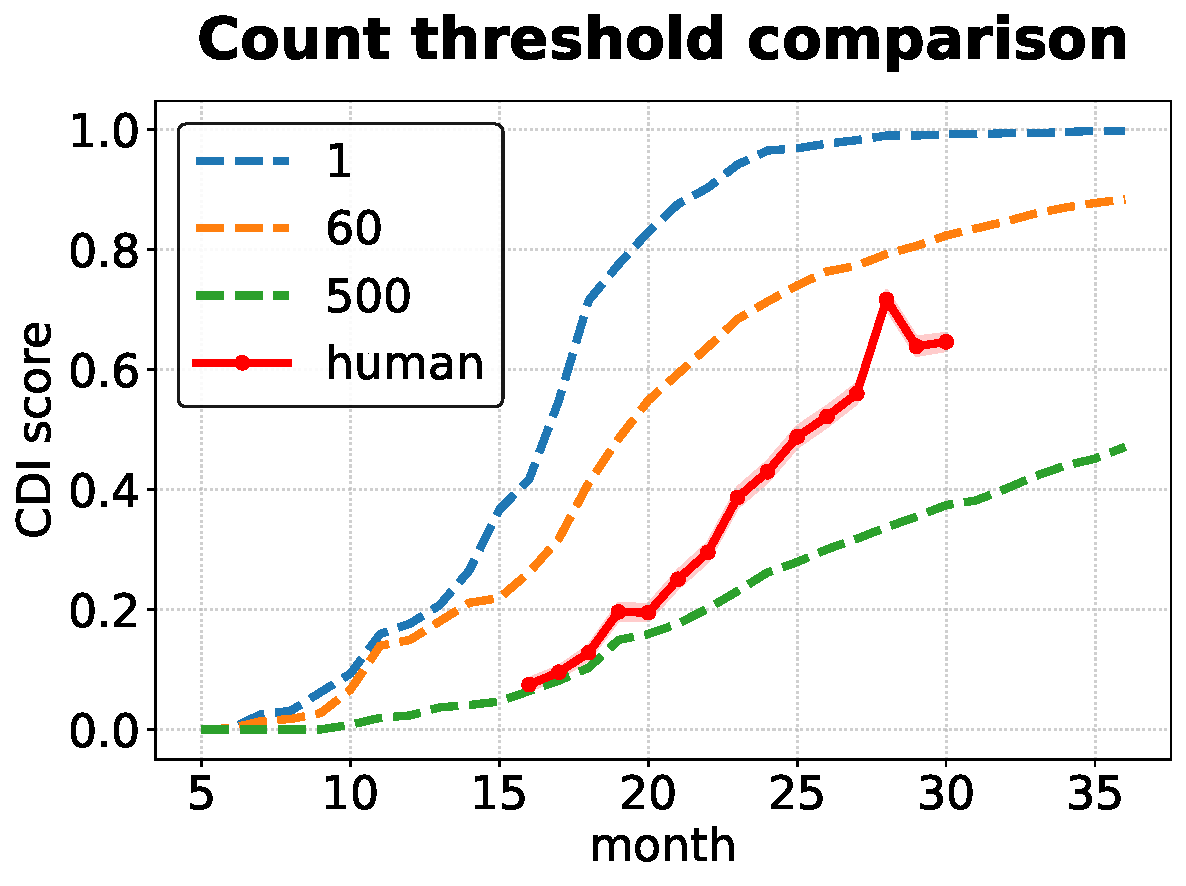
\includegraphics[width=0.5\textwidth]{fig/threshold.pdf}}
\caption{\textbf{Count-based calibration} Comparison of different word frequency thresholds for determining word acquisition. The optimal threshold (60 occurrences) was selected based on alignment with parental vocabulary size reports (red line). Each threshold produces distinct vocabulary growth trajectories, with higher thresholds resulting in more conservative estimates.}
\label{fig:threshold}
\end{figure}


Notably, the frequency effects observed in the Machine CDI are evaluated on a selected subset matched with the human-CDI set. It is unclear whether this effect is influenced by the randomness of sampling. Also, the selected words are typically in the median frequency bands, making it unknown whether such an effect stems from the limited generation size. To address this concern, we expanded our analysis of the model generations using the same and larger sampling sets. Figure~\ref{fig:distr} shows the word frequency distributions of the training and generated datasets by the LSTM model trained on 3.4M words, with different generation sizes. Expanding the generation set mitigates some truncation effects, as more high-frequency words are generated, but low-frequency words remain underrepresented. This pattern reflects the model’s limited ability to reproduce realistic word distributions, especially for rare words, even with larger sampling sizes.


\begin{figure}[ht]
\centering
\subfloat{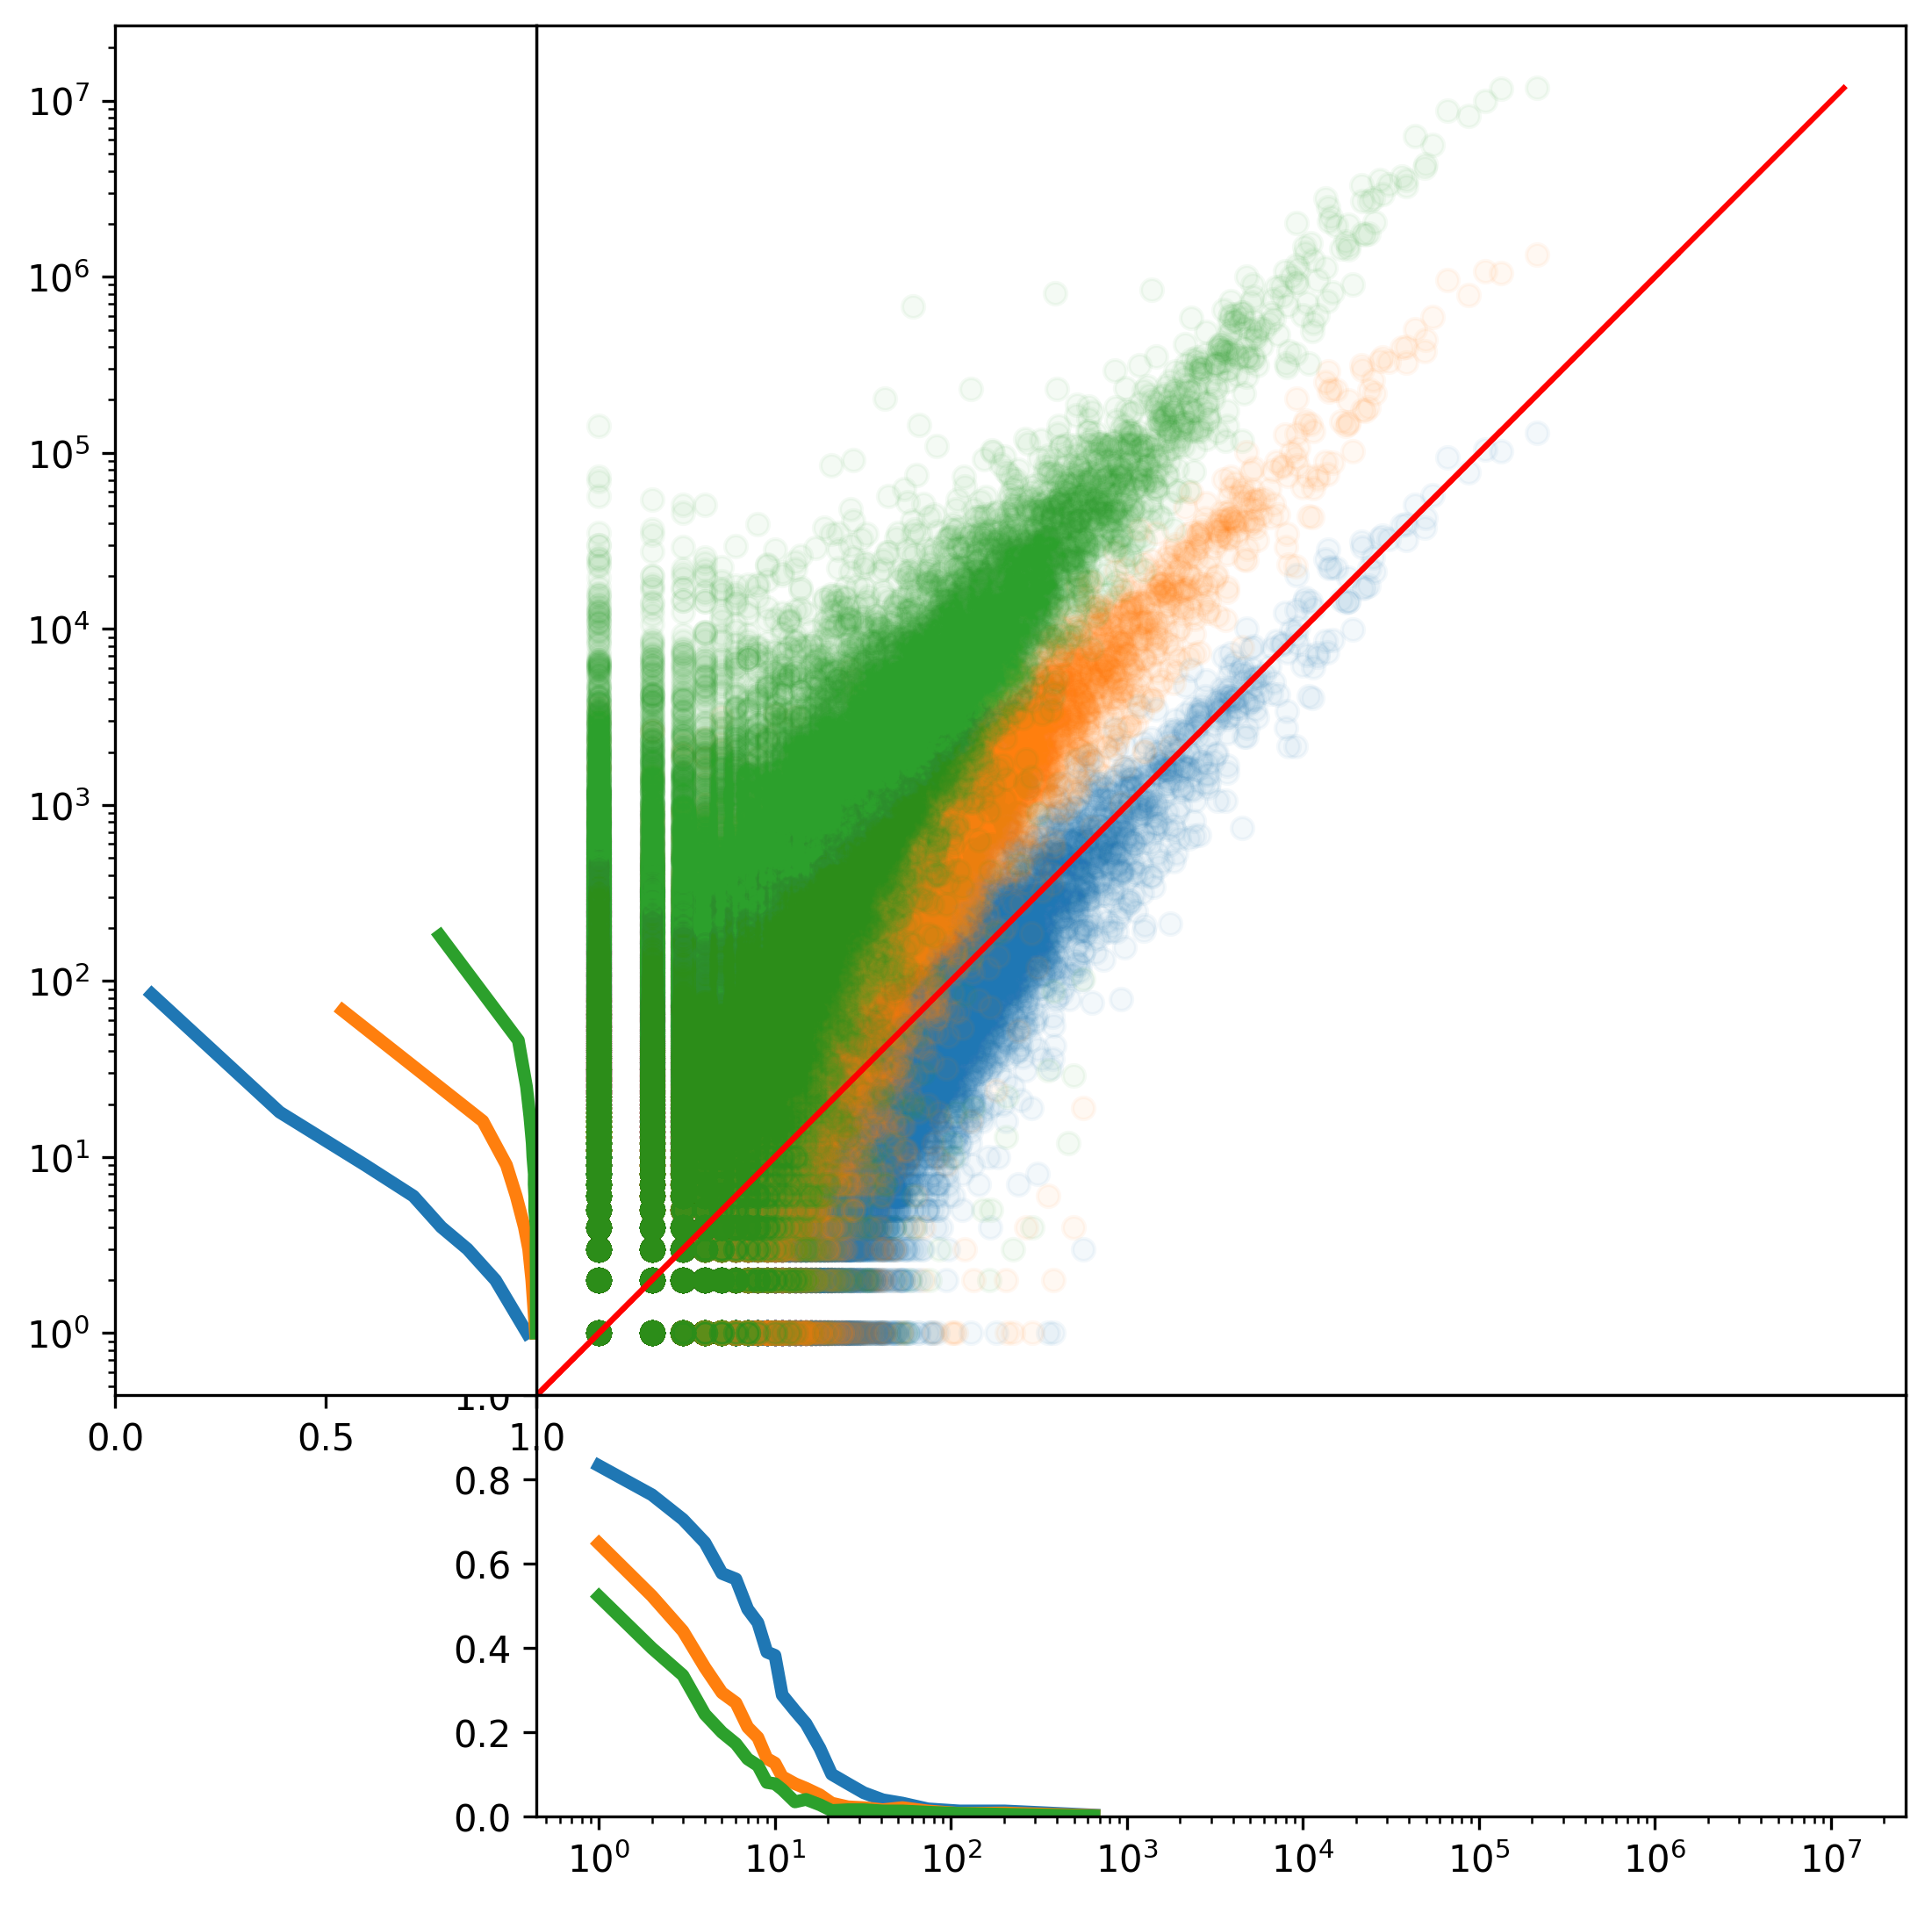
\includegraphics[width=0.3\textwidth]{fig/distr_LSTM_400.png}}
\hspace{1 pt}
\subfloat{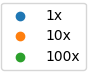
\includegraphics[width=0.1\textwidth]{fig/distr_cap.png}}
\caption{\textbf{Word count distribution(temperature = 1.0)}.Word frequency relationships between training and generation sets under different sampling conditions (1x, 10x, 100x generation volume). x-axis: word frequency in the training set; y-axis: word frequency in the generation set. Side plot on the bottom show Missing rates as a function of word count in input corpus.}
\label{fig:distr}
\end{figure}


Although models trained on higher-exposure estimates (1000 h) achieve slightly higher \meCDI{} scores than those trained on smaller sets (100 h, 500 h), the overall developmental trajectories remain similar. This pattern indicates that scaling input exposure alone does not yield more human-like developmental dynamics; instead, the gap likely arises from structural differences in learning mechanisms rather than data quantity.

\begin{figure}[ht]
\centering
\subfloat{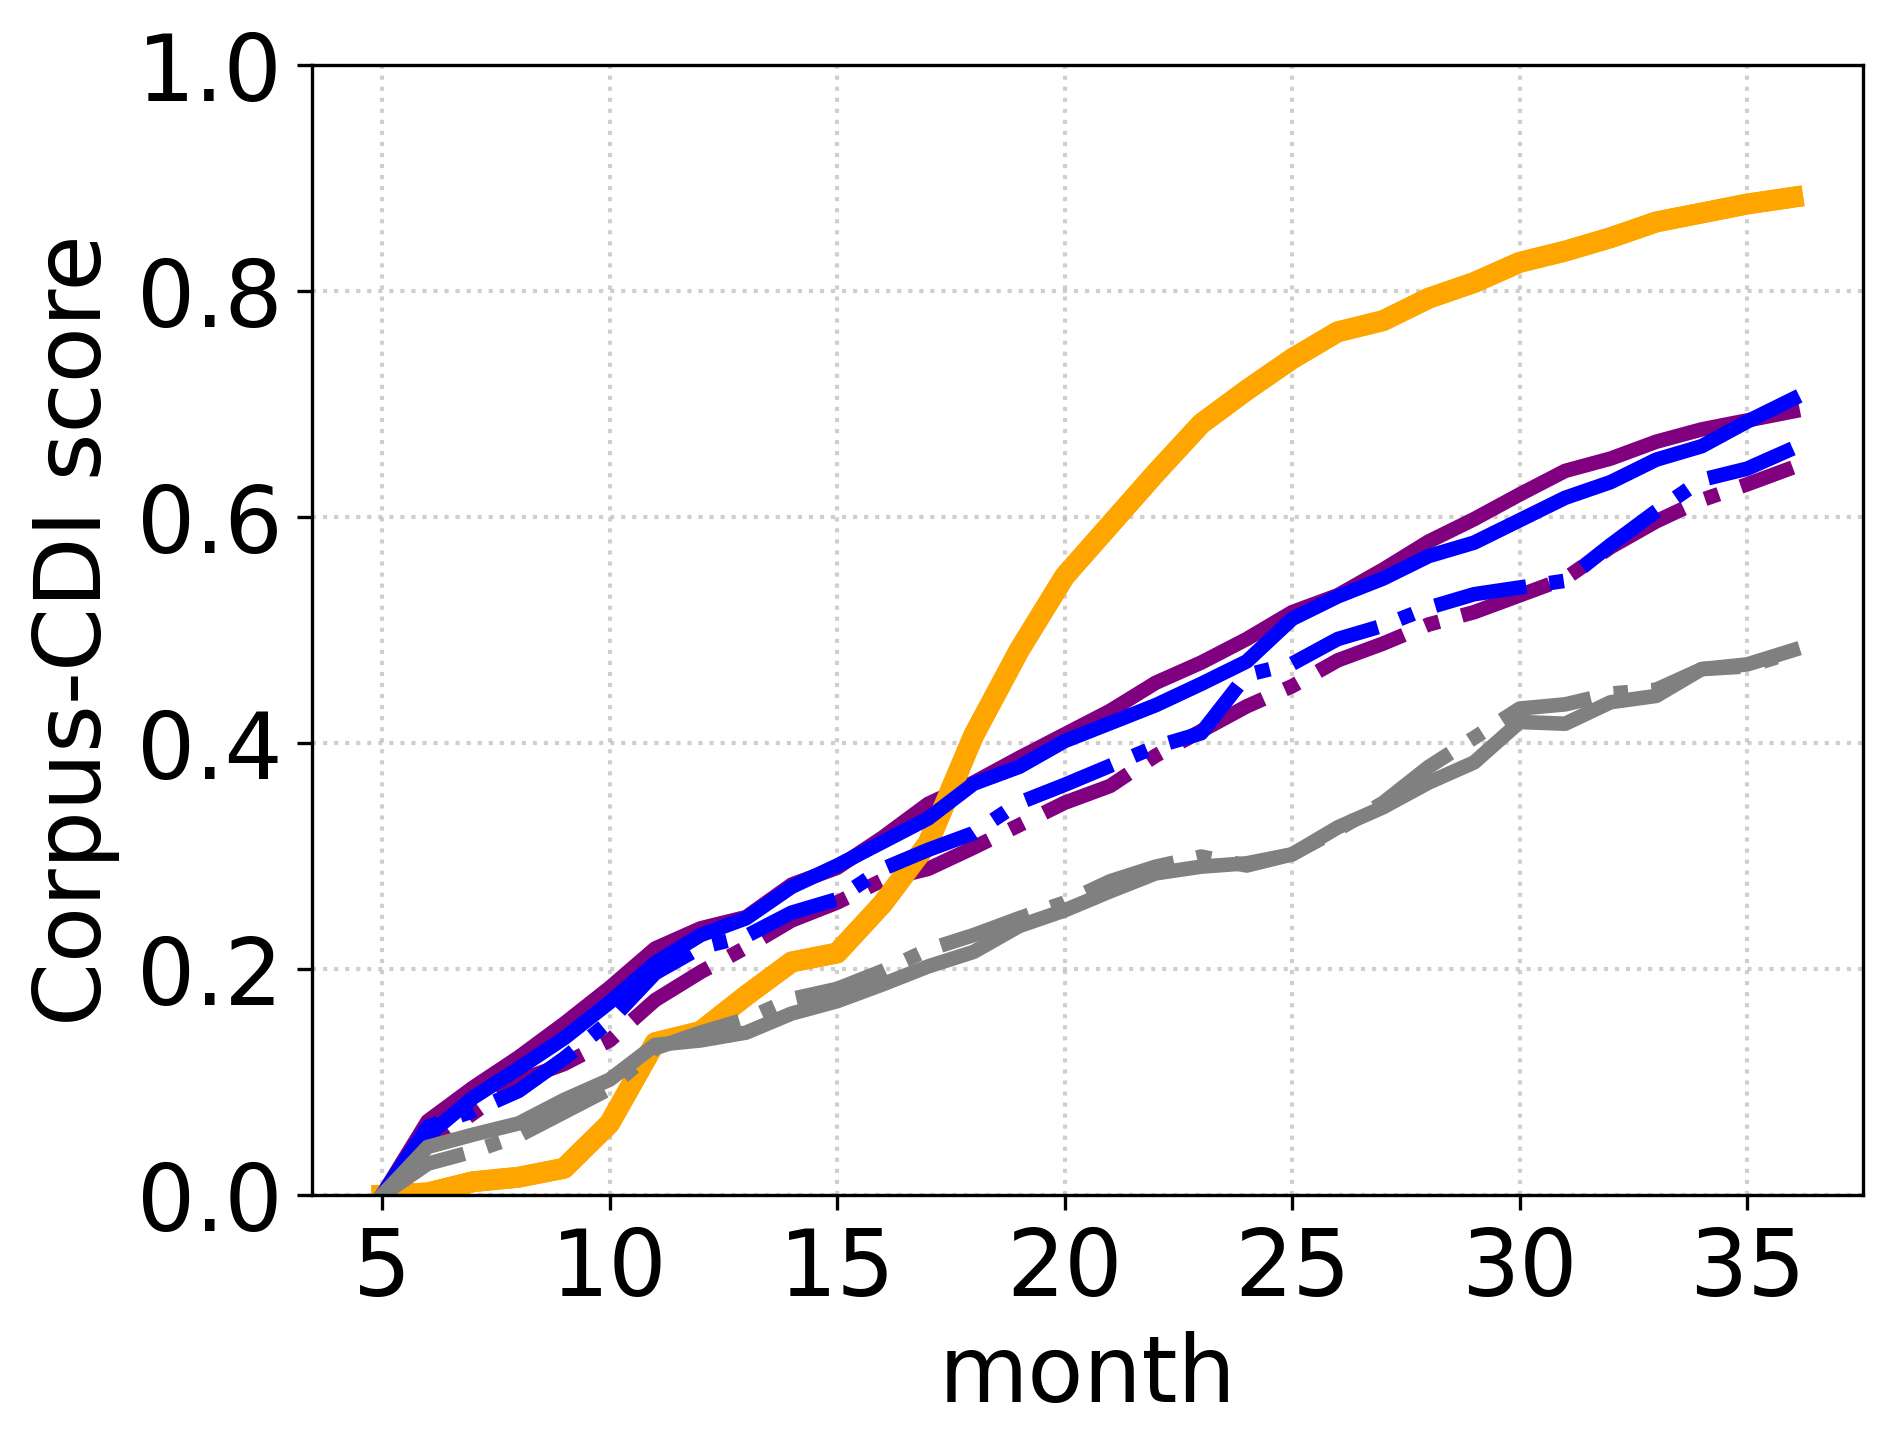
\includegraphics[width=0.35\textwidth]{fig/hour.png}}
\subfloat{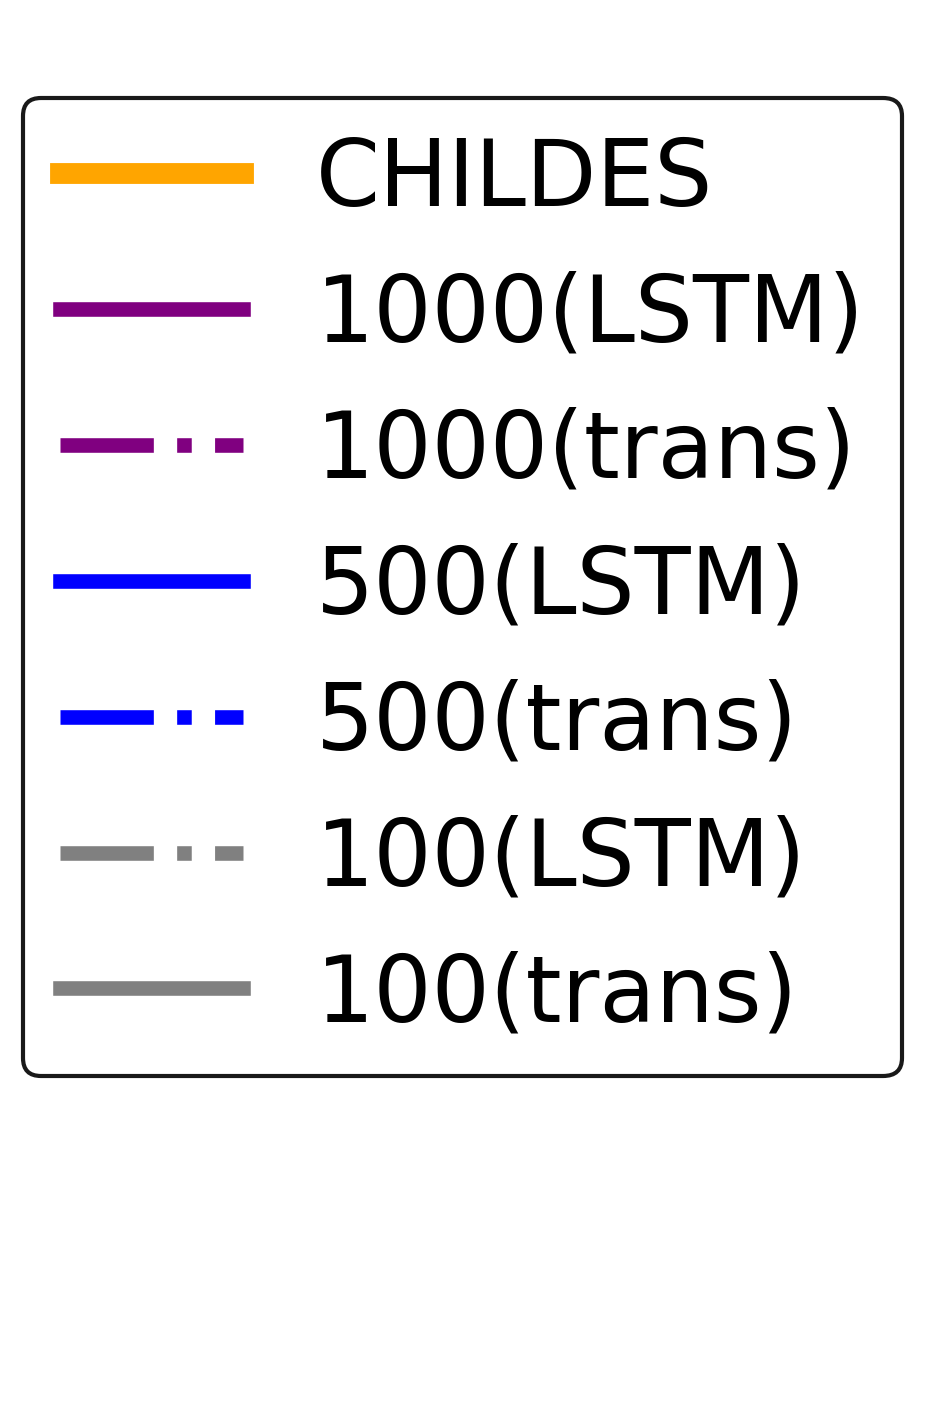
\includegraphics[width=0.1\textwidth]{fig/hour_legend.png}}
\caption{\textbf{Model vocabulary growth across estimated annual exposure levels.} Comparison of \meCDI{} trajectories for models trained on 100-, 500-, and 1000-hour exposure estimates, alongside CHILDES child production data. Models show roughly linear vocabulary growth that scales modestly with total exposure but remains far below the human developmental curve. }
\label{fig:hour}
\end{figure}

